% Options for packages loaded elsewhere
\PassOptionsToPackage{unicode}{hyperref}
\PassOptionsToPackage{hyphens}{url}
\PassOptionsToPackage{dvipsnames,svgnames,x11names}{xcolor}
%
\documentclass[
  authoryear,
  preprint,
  3p]{elsarticle}

\usepackage{amsmath,amssymb}
\usepackage{iftex}
\ifPDFTeX
  \usepackage[T1]{fontenc}
  \usepackage[utf8]{inputenc}
  \usepackage{textcomp} % provide euro and other symbols
\else % if luatex or xetex
  \usepackage{unicode-math}
  \defaultfontfeatures{Scale=MatchLowercase}
  \defaultfontfeatures[\rmfamily]{Ligatures=TeX,Scale=1}
\fi
\usepackage{lmodern}
\ifPDFTeX\else  
    % xetex/luatex font selection
\fi
% Use upquote if available, for straight quotes in verbatim environments
\IfFileExists{upquote.sty}{\usepackage{upquote}}{}
\IfFileExists{microtype.sty}{% use microtype if available
  \usepackage[]{microtype}
  \UseMicrotypeSet[protrusion]{basicmath} % disable protrusion for tt fonts
}{}
\makeatletter
\@ifundefined{KOMAClassName}{% if non-KOMA class
  \IfFileExists{parskip.sty}{%
    \usepackage{parskip}
  }{% else
    \setlength{\parindent}{0pt}
    \setlength{\parskip}{6pt plus 2pt minus 1pt}}
}{% if KOMA class
  \KOMAoptions{parskip=half}}
\makeatother
\usepackage{xcolor}
\setlength{\emergencystretch}{3em} % prevent overfull lines
\setcounter{secnumdepth}{5}
% Make \paragraph and \subparagraph free-standing
\makeatletter
\ifx\paragraph\undefined\else
  \let\oldparagraph\paragraph
  \renewcommand{\paragraph}{
    \@ifstar
      \xxxParagraphStar
      \xxxParagraphNoStar
  }
  \newcommand{\xxxParagraphStar}[1]{\oldparagraph*{#1}\mbox{}}
  \newcommand{\xxxParagraphNoStar}[1]{\oldparagraph{#1}\mbox{}}
\fi
\ifx\subparagraph\undefined\else
  \let\oldsubparagraph\subparagraph
  \renewcommand{\subparagraph}{
    \@ifstar
      \xxxSubParagraphStar
      \xxxSubParagraphNoStar
  }
  \newcommand{\xxxSubParagraphStar}[1]{\oldsubparagraph*{#1}\mbox{}}
  \newcommand{\xxxSubParagraphNoStar}[1]{\oldsubparagraph{#1}\mbox{}}
\fi
\makeatother


\providecommand{\tightlist}{%
  \setlength{\itemsep}{0pt}\setlength{\parskip}{0pt}}\usepackage{longtable,booktabs,array}
\usepackage{calc} % for calculating minipage widths
% Correct order of tables after \paragraph or \subparagraph
\usepackage{etoolbox}
\makeatletter
\patchcmd\longtable{\par}{\if@noskipsec\mbox{}\fi\par}{}{}
\makeatother
% Allow footnotes in longtable head/foot
\IfFileExists{footnotehyper.sty}{\usepackage{footnotehyper}}{\usepackage{footnote}}
\makesavenoteenv{longtable}
\usepackage{graphicx}
\makeatletter
\def\maxwidth{\ifdim\Gin@nat@width>\linewidth\linewidth\else\Gin@nat@width\fi}
\def\maxheight{\ifdim\Gin@nat@height>\textheight\textheight\else\Gin@nat@height\fi}
\makeatother
% Scale images if necessary, so that they will not overflow the page
% margins by default, and it is still possible to overwrite the defaults
% using explicit options in \includegraphics[width, height, ...]{}
\setkeys{Gin}{width=\maxwidth,height=\maxheight,keepaspectratio}
% Set default figure placement to htbp
\makeatletter
\def\fps@figure{htbp}
\makeatother

\usepackage{booktabs}
\usepackage{longtable}
\usepackage{array}
\usepackage{multirow}
\usepackage{wrapfig}
\usepackage{float}
\usepackage{colortbl}
\usepackage{pdflscape}
\usepackage{tabu}
\usepackage{threeparttable}
\usepackage{threeparttablex}
\usepackage[normalem]{ulem}
\usepackage{makecell}
\usepackage{xcolor}
\makeatletter
\@ifpackageloaded{caption}{}{\usepackage{caption}}
\AtBeginDocument{%
\ifdefined\contentsname
  \renewcommand*\contentsname{Table of contents}
\else
  \newcommand\contentsname{Table of contents}
\fi
\ifdefined\listfigurename
  \renewcommand*\listfigurename{List of Figures}
\else
  \newcommand\listfigurename{List of Figures}
\fi
\ifdefined\listtablename
  \renewcommand*\listtablename{List of Tables}
\else
  \newcommand\listtablename{List of Tables}
\fi
\ifdefined\figurename
  \renewcommand*\figurename{Figure}
\else
  \newcommand\figurename{Figure}
\fi
\ifdefined\tablename
  \renewcommand*\tablename{Table}
\else
  \newcommand\tablename{Table}
\fi
}
\@ifpackageloaded{float}{}{\usepackage{float}}
\floatstyle{ruled}
\@ifundefined{c@chapter}{\newfloat{codelisting}{h}{lop}}{\newfloat{codelisting}{h}{lop}[chapter]}
\floatname{codelisting}{Listing}
\newcommand*\listoflistings{\listof{codelisting}{List of Listings}}
\makeatother
\makeatletter
\makeatother
\makeatletter
\@ifpackageloaded{caption}{}{\usepackage{caption}}
\@ifpackageloaded{subcaption}{}{\usepackage{subcaption}}
\makeatother
\journal{the Journal of Futures Markets}

\ifLuaTeX
  \usepackage{selnolig}  % disable illegal ligatures
\fi
\usepackage[]{natbib}
\bibliographystyle{elsarticle-harv}
\usepackage{bookmark}

\IfFileExists{xurl.sty}{\usepackage{xurl}}{} % add URL line breaks if available
\urlstyle{same} % disable monospaced font for URLs
\hypersetup{
  pdftitle={Financialisation of Commodity Markets},
  pdfauthor={Devraj Basu; Olivier Bauthéac},
  pdfkeywords={Commodity markets, Financialisation, Co-movement, Asset
pricing},
  colorlinks=true,
  linkcolor={blue},
  filecolor={Maroon},
  citecolor={Blue},
  urlcolor={Blue},
  pdfcreator={LaTeX via pandoc}}


\setlength{\parindent}{6pt}
\begin{document}

\begin{frontmatter}
\title{Financialisation of Commodity Markets \\\large{Co-movement
Behind-the-Scenes} }
\author[1]{Devraj Basu%
\corref{cor1}%
}
 \ead{devraj.basu@strath.ac.uk} 
\author[1]{Olivier Bauthéac%
%
}
 \ead{olivier.bautheac@strath.ac.uk} 

\affiliation[1]{organization={University of Strathclyde Business
School, Accounting \& Finance},addressline={199 Cathedral
Street},city={Glasgow},postcode={G4 0QU},postcodesep={}}

\cortext[cor1]{Corresponding author}


        
\begin{abstract}
In the early 2000s institutional investors entered the commodity futures
markets en masse with passive, long only, index type positions in sharp
contrast with those typically assumed by traditional expert
participants. A heated public debate soon erupted over the perceived
consequences of the phenomenon---commonly referred to as
``financialisation''---and, in response to immediate policy concerns,
the matter was thrust onto the academic sphere as a burning issue. With
the benefit of hindsight it now seems that the academic debate was
framed rather narrowly, used contentious research methods, and
eventually led to regulatory changes that were therefore perhaps
unwarranted. In contrast, we take a broader approach where we consider a
large cross-section of liquid commodities as suggested by the nature of
financialisation that comprehends commodity futures as an asset class.
We examine the cross-sectional interconnectedness of these assets and
uses a bespoke asset pricing factors based framework to study the issue
through the lens of co-movement. We find that the phenomenon had
ontological consequences for the commodity complex with its impact
extending beyond the mechanical effects induced by indexation. The onset
of the financial crisis and the monetary policy regimes that followed,
on the other hand, seem to have set off a motion of reversion to legacy
pre-financialisation fundamentals.
\end{abstract}





\begin{keyword}
    Commodity markets \sep Financialisation \sep Co-movement \sep 
    Asset pricing
\end{keyword}
\end{frontmatter}
    

\newpage

\setlength{\parindent}{0pt}

\section{Introduction}\label{sec-introduction}

The last twenty years have seen major upheavals in the commodity markets
with the onset of financialisation\footnote{Starting around 2004, with a
  view of commodity markets as an emerging asset class and in an effort
  to hedge against inflation and seek diversification benefits
  \citep{buyuksahin_speculators_2014, singleton_investor_2013},
  institutional investors sent forth an unprecedented flow of capital
  into commodity futures markets. This phenomenon is commonly referred
  to as the financialisation of commodities
  \citep{domanski_financial_2007}.} as well as the period of the 2008
financial crisis and its aftermath. Financialisation appears to have
affected multiple economic sectors, including agriculture and energy,
and its impact has been hotly debated in the policy, legislative,
regulatory, and academic spheres. A rigorous legislative scrutiny
accompanied by a vigorous policy and academic debate across a number of
disciplines about the perceived effects on commodity prices of the
unprecedented inflow of institutional funds brought into commodity
futures markets by new index type investors\footnote{See section
  Section~\ref{sec-background} for a detailed discussion.} eventually
led to regulatory changes in several individual markets.\\
In response to immediate policy concerns, the academic debate was
initially framed rather narrowly around adequacy of speculation---the
burning issue of the day---at the individual commodity level and the
ensuing academic analysis focused on the more mechanical effects of
financialisation. With the benefit of hindsight, this approach seems to
lack a fundamental understanding of the phenomenon it endeavoured to
study and which consequences it attempted to address.\\
Financialisation was a phenomenon global in nature that, through the
channel of index investment, affected the whole cross-section of liquid
commodities at once, eventually spurring its transition away from a
collection of idiosyncratic markets to its emergence as an asset class.
Focusing on individual markets in this context thus seems limited. Most
of the studies underpinning the regulatory response to financialisation
took the form of pairwise correlation, causation and to some extent
co-integration analysis, all of which are idiosyncratic in nature for
they study single pairs of individual assets. Besides, some of these
techniques since proved controversial and seem to produce results the
quality of which may fall short of the standards that may reasonably be
expected to lay the ground for legislative action. Although appealing,
for it comes with the promise of prompt ``significant'' results, this
approach misses a critical corollary of the substantial advent of a new
category of players in a (set of) market(s): the alteration of
fundamentals it potentially induces, best observed in this context
through the lens of commercial hedging pressure
\citep{keynes_treatise_1930, hicks_value_1939}.\\
While essential to the understanding of the phenomenon, the global
nature of financialisation and its impact on market fundamentals
therefore appear to have been originally overlooked and another
approach, perhaps more refined, seems warranted.

\medskip

We strive to provide one in this study by taking a fundamentally
different empirical perspective that is broader in scope. We examine the
interconnectedness of the commodity complex at the cross-sectional
level, considering the entire cross-section of actively traded
commodities on futures markets and use a bespoke futures-based asset
pricing framework that includes factors constructed using both
theoretical fundamentals and liquidity considerations.\\
The global nature of financialisation makes cross-sectional co-movement
a cornerstone issue that the direct impact of increased market
participation alone might not be able to fully explain for it
potentially had deeper effects, for example on market fundamentals as
our results suggest. Commodity futures markets have a history of being
the classic physical commodity price risk shifting conduit for commodity
specialists. Over the financialisation period we observe a decrease in
effectiveness of commercial hedging pressure (CHP) at explaining
commodity futures returns at the individual level accompanied by a more
pronounced increase at the aggregate level. We further note an overall
shift in the nature of hedger's behaviour away from the traditional
Keynesian view of risk transfer with higher individual risk premiums
over phases of cross-sectional contango as opposed to backwardation.
Both patterns suggest that the phenomenon may have altered this
long-standing paradigm of commercial risk transfer with the entry of
long only commodity index traders (CITs) with very different demands
from traditional participants. This change could have altered the
hedging ontology in these markets and our asset pricing framework is
tailored to detect these more subtle effects driven by changes in the
nature of market participation.\\
Factor model techniques are well suited to isolating common driving
factors and detecting co-movement
\citep{fama_common_1993, carhart_persistence_1997, asness_devil_2013, fama_five_factor_2015, hou_digesting_2015, asness_fact_2015, frazzini_betting_2014, asness_quality_2019}
at a broader level, beyond individual pairs of assets, and are commonly
used to study commodity market fundamentals
\citep{schwartz_short_2000, miffre_momentum_2007, gorton_fundamentals_2012, cortazar_commodity_2013, yang_investment_2013, daskalaki_factors_2014, szymanowska_anatomy_2014, fernandez_skewness_2018, bakshi_understanding_2019, boons_basis_2019, sakkas_factor_2020};
they consequently seem well adapted to study these two issues
simultaneously. Building on theory we therefore develop a bespoke
commodity-based asset pricing framework comprised of factor models based
both on fundamentals as well as liquidity considerations.\\
One of these is based on the Keynes-Hicks
\citep{keynes_some_1923, keynes_treatise_1930, hicks_value_1939, hicks_value_1946}
risk transfer approach to the term structure; the corresponding ``theory
of normal backwardation'', complemented for the possibility of contango
\citep{houthakker_restatement_1957, cootner_returns_1960}, postulates
that futures prices for a given commodity are inversely related to the
extent that commercial hedgers are short or long and using commercial
hedging pressure (CHP) as a proxy for hedgers net market position we
construct factor mimicking portfolios that capture the impact of hedging
pressure as a systemic factor \citep{basu_capturing_2013}. The
cross-sectional nature of financialisation
\citep{cheng_financialisation_2014, basak_model_2016} further leads us
to extend this paradigm by incorporating aggregate CHP (\textbf{CHP}), a
market wide measure of hedging pressure first considered in
\citet{hong_what_2012}. In this context, returns for individual
commodities should be high in periods where \textbf{CHP} is low
(\textbf{backwardation}) and low in periods where \textbf{CHP} is high
(\textbf{contango}). Working's contending approach that relates futures
price formation to storage costs in the theory of ``the price of
storage'' \citep{working_theory_1949} forms the basis of another model
that we consider where, following \citet{szymanowska_anatomy_2014} and
\citet{fuertes_commodity_2015} who demonstrate that the term structure
factor has explanatory power for the cross-section of commodity returns,
we construct factor mimicking portfolios using roll-yield as a proxy for
the front end shape of individual commodity term structures. We further
consider a liquidity-based model following \citet{hong_what_2012} who
find that open interest growth has predictive power for individual
commodity returns and again, using the latter measure as a proxy for
individual commodity liquidity, we construct long-short factor mimicking
portfolios.\\
We study the performance of these models on a set of twenty-four US
traded commodities and six GB traded (London Metal Exchange) base metals
over the 1997/2018 period that we divide into four distinct sub-periods:
pre-financialisation (1997/2003); financialisation
(2004/2008\footnote{Starting point based on earlier studies
  \citep{baker_financialization_2021, christoffersen_factor_2014}.});
financial crisis and aftermath, including loose monetary policy regimes
that followed (2008/2013); and post-crisis (2014-2018).

\bigskip
\bigskip

Consistent with earlier studies, we observe that mean returns for the US
traded commodities are sharply higher over the financialisation period
compared to pre-financialisation with the pattern extending to GB traded
metals.\\
Over the first period the cross-sectional average returns during phases
of \textbf{backwardation} for both the US and GB commodities are
positive and overall higher than during phases of \textbf{contango},
providing broad support for an aggregate version of the Keynesian
hedging pressure hypothesis. Over the second period this pattern
reverses, with both the US and GB commodities having higher returns
during phases of \textbf{contango} as opposed to \textbf{backwardation}.
This change in pattern suggests the onset of financialisation altered
the traditional risk shifting nature of hedger's behaviour, implied by
the Keynesian hypothesis.\\
This change of paradigm due to the arrival of financial investors, on
the other hand, raises the question of whether they functioned as
liquidity providers or demanders. Arguments have been put forward in
favour of both possibilities with \citet{moskowitz_time_2012} arguing
that financial investors provide liquidity and \citet{kang_tale_2020}
taking the opposite stance. Our analysis of individual commodity
returns' relation with both CHP and \textbf{CHP} before and during
financialisation sheds a new light on this issue with our results
suggesting that financial investors may have been liquidity demanders
leading hedgers to become liquidity providers.

\medskip

These entered the commodity spectrum en masse with across-the-board
index type positions prompting the transition of the complex from a
collection of idiosyncratic markets towards a more cohesive ensemble
akin to an asset class. In this context of heightened cross-asset market
participation the issue of interconnectedness stands out as paramount
and we strive to investigate it by first examining the correlation
structure of our sample set of assets at the global, country, sector and
sub-sector levels. Our results indicate higher interdependence within
the full cross-section of commodities over the financialisation period,
consistent with both the empirical and theoretical literature. The
increase appears to be driven by the US metals sector, a new observation
to the best of our knowledge, and, unlike individual commodity returns,
does not seem to be regime-driven, as a similar pattern of results is
observed across phases of \textbf{backwardation} and \textbf{contango}.

\medskip

\citet{goldstein_speculation_2014} and \citet{goldstein_commodity_2022}
argue that the arrival of financial investors had an impact on the
extent of normal backwardation in commodity futures markets. Based on
their analysis we would expect our average CHP factor, based on
backwardation as measured by hedger's positions (Keynesian perspective,
theory of normal backwardation: \citet{keynes_treatise_1930},
\citet{hicks_value_1939}, \citet{houthakker_speculators_1957},
\citet{telser_futures_1958}), as well our term structure factor, based
on backwardation as measured by roll yield (Working's perspective,
theory of storage: \citet{working_price_1933},
\citet{kaldor_speculation_1939}, \citet{working_theory_1948},
\citet{brennan_supply_1958}, \citet{cootner_returns_1960},
\citet{weymar_supply_1966}, \citet{danthine_information_1978},
\citet{turnovsky_determination_1983}, \citet{schwartz_stochastic_1997}),
to be best suited to measure the impact of financialisation.\\
We analyse the pricing dynamics over the different periods by first
studying the time series explanatory performance of the various factors
on our commodity assets sample. The market-based factor outperforms the
other three in the first period and, although its performance increases
over the financialisation period, that of the CHP factor shows a greater
improvement in a relative sense. The performance of the market factor is
driven by agricultural and energy commodities in the first period while
metals strongly contribute to the performance improvement observed over
the second period. The sector is also the driving force behind the
dramatic improvement of the CHP factor during financialisation, led by
its long leg on which metals predominantly load. The sector is similarly
responsible for the improved performance of the short leg of the term
structure factor of the period, on which the metals also predominantly
load. Taken together, these results provide evidence of convergence of
Keynesian and Working's theories of the term structure in detecting
price co-movement during financialisation and strongly suggest that the
term structure related attributes (hedging pressure/roll) co-movement
and price co-movement link was concentrated in the metals sub-sector.\\
The GB traded base metals provide a useful set of assets to test how
widespread were the changes in pricing dynamics brought about by the
onset of financialisation. To that end, we examine the performance of
the four factors on the six GB metals; the results show that there was
co-movement in global metals returns in the second period and that this
co-movement could be detected by our term structure related models,
particularly so by our hedging pressure-based model.

\bigskip

The onset of the financial crisis and the monetary policy regimes that
followed, on the other hand, also appear to have induced significant
changes. Commodity futures returns fell dramatically while the symmetry
between the dynamics of CHP and \textbf{CHP}'s' explanatory power on
individual commodity returns breaks with both now seemingly converging.
The correlation structure is also affected with evidence of an
intensification of the higher interdependence within the full
cross-section of commodities prompted by financialisation, consistent
with the greater interdependence between equity and commodity markets
over the period documented in the literature. The pricing results
further indicate the emergence of a systematic factor across the entire
cross-section of the US commodities as well as evidence of cross-market
linkages with the GB traded commodity subset. The onset of the financial
crisis thus seems to have had a global impact on the commodity complex
in contrast with financialisation, much more closely related to the
metals sector.

\medskip

The returns pull-back continues into the post-crisis period,
interestingly amidst a lower volatility environment, suggesting that the
underlying contributing factors--including investment outflows from the
commodity futures complex as well as perhaps the evolving nature of
global oil demand over the period--have had a lower impact on volatility
than witnessed during financialisation. The pattern of reversion toward
the pre-financialisation Keynesian paradigm continues stronger with mean
returns higher during phases of \textbf{backwardation} relative to
\textbf{contango} and the difference more pronounced than over the
crisis period. In contrast to the crisis period when they seemed to be
converging, the pricing performance of CHP and \textbf{CHP} now part
ways, seemingly reverting to the Keynesian paradigm observed
pre-financialisation, further suggesting a reversion to legacy commodity
specific dynamics. The pull back extends to the correlation structure
with an across-the-board decrease in average pairwise correlations down
to levels below those observed during financialisation. The average
market factor beta for the entire cross-section shows a similar pattern,
dropping down below the level observed during financialization with the
decline seemingly driven by the metals sector, particularly the GB
traded segment. The pattern extends to the pricing performance of all
factors that drops below levels observed during financialisation.\\
Moreover, both the average correlations and the pricing performance of
the market factor are considerably stronger during \textbf{contango}
phases, unlike previous periods, which showed no substantial difference
between regimes with the pattern particularly pronounced for metal
assets globally, both US and GB traded. These results document the
emerging role/dominance of the \textbf{contango} regime post-crisis and
could provide a valuable basis for further research.

\bigskip
\bigskip

Financialisation was an issue of such policy importance that it
triggered legislative action. The debate was initially framed around
adequacy of speculation, the burning issue of the day, and the ensuing
academic analysis focused on the more mechanical effects of
financialisation.\\
With the benefit of hindsight, it appears this approach was perhaps too
narrow, and it now seems necessary to address the phenomenon from a
broader perspective. Commodity price dynamics appear to have altered
substantially in quite different ways over the financialisation and the
financial crisis periods and both our cross-sectional approach to
examining interconnectedness in the complex as well as our commodity
futures asset pricing framework together seem able to provide new
insights into the nature of these changes: financialisation was a
phenomenon endogenous to the commodity markets transmitted via the
commodity futures markets and which effects were particularly strong for
the metals sector while the crisis and its aftermath seem to have
delivered an exogenous shock across the entire cross-section of liquid
commodities, further altering the cross-sectional dynamics, and
potentially triggering a reversion to pre-financialisation dynamics in
the most recent period.

The initial view of financialisation was that it consisted of
speculative flows which had the effect of driving up and creating bubble
like conditions in commodity futures prices\footnote{\citet{masters_testimony_2008};
  \citet{masters_accidental_2008}; \citet{unctad_global_2009};
  \citet{deschutter_food_2010}; \citet{gilbert_how_2010};
  \citet{gilbert_speculative_2010}; \citet{herman_not_2011};
  \citet{schumann_hunger_2011}; \citet{singleton_investor_2013}.}.
However, the fundamental question of the nature of the impact of
financialisation across the entire cross-section of commodity futures
markets has not yet been completely answered. We provide an empirical
complement to a new stream of theoretical studies that try to model the
impact of financialisation on various aspects of commodity futures
markets\footnote{\citet{etula_broker-dealer_2013},
  \citet{acharya_limits_2013}, \citet{cheng_convective_2014},
  \citet{leclercq_equilibrium_2014}, \citet{sockin_informational_2015},
  \citet{goldstein_speculation_2014}, \citet{ekeland_speculation_2014},
  \citet{goldstein_commodity_2022}, \citet{ekeland_hedging_2019},
  \citet{isleimeyyeh_role_2020}.} and demonstrate that the effects of
financialisation extend beyond the mechanical effects induced by
indexation as outlined in \citet{tang_index_2012} and
\citet{basak_model_2016}.

\newpage

\section{Data \& methods}\label{sec-data-methods}

\subsection{Background}\label{sec-background}

The period from 1998 to 2008 saw an influx of investment into commodity
index linked products most of which made its way into the commodity
futures market. Popular commodity indexes whose goal was to track the
broad movement of commodity prices became accessible by means of swaps,
exchange traded funds and exchange traded notes and attracted at least
\$100 billion of net super-hoc investment over the 1998-2008 period.

\medskip

Concerns over the consequences of this financialisation phenomenon
eventually led to legislative changes including the approval of Rule 76
FR 4752 issued by the US Commodity Futures Trading Commission (CFTC) on
January 26\textsuperscript{th}, 2011. This provision emanates from the
Dodd-Frank Wall Street and Consumer Protection Act of 2010 (Title VII,
Section 737) that mandates the CFTC to use position limits to restrict
the flow of speculative capital into a number of commodity markets. The
Rule was approved in a close 3-2 vote and the ensuing rule-making
process was extremely contentious with several commissioners (Michael
Dunn and Scott D. O'Malia in particular) expressing reservations about
the lack of supporting evidence and the Rule also triggering thousands
of comment letters as well as a lawsuit against the CFTC spearheaded by
two Wall Street trade groups, the International Swaps \& Derivatives
Association (ISDA) and the Securities Industries \& Financial Markets
Association (SIFMA)\footnote{ISDA \& SIFMA v US CFTC; Complaint,
  1:11-cv-02146; December 2\textsuperscript{nd}, 2011.}.

\medskip

A world-wide debate ensued about the role of index funds in commodity
markets. The first responses to the 2007/2008 crisis of escalating food
and energy prices took the form of policy reports, many of which
reasoned that the growth of commodity index funds came along with an
influx of largely speculative capital that was responsible for driving
commodity prices beyond their historic highs
\citep{deschutter_food_2010, gilbert_speculative_2010, herman_not_2011, schumann_hunger_2011, unctad_global_2009}.\\
Early US Senate investigations on the matter drew on pricing and trading
data supplied by the CFTC as well as interviews with numerous experts
including hedge fund manager Michael Masters who linked the growing
presence of index investors in US agricultural and energy markets to the
observed surges in both futures and cash prices
\citep{masters_testimony_2008, masters_accidental_2008}. This contention
has since come to be known as the ``Masters' hypothesis'' and was
largely endorsed by the final US Senate report on the issue
\citep{senate_excessive_2009}.\\
At this stage, the question thrust on the academic sphere was whether
``excessive speculation''\footnote{Understood as the market activity
  peculiar to index type investors.} was linked to escalating energy and
agricultural commodity prices. A number of ensuing academic studies,
most of which used commodity specific correlation and causality based
analysis have since disproved this contention: \citet{irwin_devil_2009},
\citet{sanders_adequacy_2010}, \citet{sanders_impact_2011},
\citet{sanders_new_2011}, \citet{irwin_commodity_2013},
\citet{brunetti_commodity_2014}, \citet{hamilton_effects_2015} and
\citet{bruno_financialisation_2017} investigated the issue in the
context of the agricultural markets; meanwhile,
\citet{buyuksahin_speculators_2011}, \citet{tokic_speculation_2012},
\citet{fattouh_role_2013}, \citet{kilian_role_2014},
\citet{knittel_simple_2016} and \citet{manera_modelling_2016} examined
the energy markets while \citet{bohl_does_2013}, \citet{kim_does_2015}
and \citet{boyd_prevalence_2016} studied both energy and agricultural
markets and \citet{irwin_index_2011},
\citet{irwin_financialisation_2012} as well as
\citet{stoll_commodity_2011} examined the commodity markets in general.
Other studies have underlined various alterations in commodity pricing
dynamics over the period. \citet{gilbert_role_2014} reject the view that
financialisation has not had any effects in the grains markets and
demonstrate that trades originated by financial market participants, and
specifically index investors, can move prices but tend to be typically
volatility-reducing. \citet{juvenal_speculation_2015} contend that the
oil price increase between 2004 and 2008 was mainly driven by the
strength of global demand but that the financialisation process of
commodity markets also played a role. Likewise,
\citet{henderson_new_2015} show that non-information-based financial
investments have important impacts on commodity prices.
\citet{cheng_financialisation_2014}, on the other hand, show that in the
case of index commodities, financialisation has transformed the risk
sharing, and information discovery functions of commodity futures
markets.

\subsection{Data}\label{sec-data}

Commodity index swaps, commodity index funds (CIFs), commodity-based
exchange traded funds (ETFs) and notes (ETNs) or commodity linked notes
(CLNs) were amongst the main investment vehicles that allowed
institutional and retail investors to build up commodity exposure in the
early 2000s
\citep{boons_stock_2012, henderson_new_2015, irwin_index_2011, unctad_global_2009, schumann_hunger_2011}.
Most of these products were primarily designed to track prominent
commodity indexes among which the S\&P-GSCI, the most popular.\\
Most of its constituents at the time of writing form the basis of the
broad cross-section of commodities that we consider in this study:
corn-\#2 yellow (XCBT), oats (XCBT), soybean meal (XCBT), soybean oil
(XCBT), soybeans (XCBT), wheat-SRW (XCBT), cattle-feeder (XCME),
cattle-live (XCME), lean hogs (XCME), cocoa (IFUS), coffee-C (IFUS),
cotton-\#2 (IFUS), lumber (XCME), orange juice (IFUS), sugar-\#11
(IFUS), natural gas (XNYM), crude oil-WTI (XNYM), gasoline (XNYM),
heating oil (XNYM), copper (XCEC), gold (XCEC), palladium (XNYM),
platinum (XNYM) and silver (XCEC). Unleaded gasoline, the NYMEX legacy
contract for gasoline, stopped trading in 2006 when it was replaced by
Reformulated Gasoline Blendstock for Oxygen Blending (RBOB) with the two
futures series trading alongside for most of the year. For our NYMEX
gasoline data series, we consider unleaded gasoline up to September
1\textsuperscript{st}, 2006 and RBOB gasoline thereafter, date at which
liquidity for the latter overtook that for the former.\\
We also consider the GB metal complex with aluminium (XLME), copper
(XLME), lead (XLME), nickel-primary (XLME), tin-refined (XLME) and zinc
(XLME). This sample cross-section of assets is further divided into
groups for the purpose of the analysis by country (US, GB), sector
(agriculturals, energy, metals) and by sub-sector (agriculturals:
grains, livestock, softs; energy: gas, petroleum; metals: base,
precious)\footnote{See Table~\ref{tbl-assets-taxonomy} for a detailed
  taxonomy of the commodity assets considered in the study.}.

\medskip

The commodity futures trading commission (CFTC) operates a comprehensive
system of collecting information on market participants known as the
large trader reporting program (LTRP) where it records and reports to
the public position data on market participants who have position levels
in excess of a particular market specific threshold\footnote{Current
  reporting level thresholds available at:
  \href{https://www.ecfr.gov/cgi-bin/retrieveECFR?gp=&SID=970471b8455f4bab7db4110cfde50731&mc=true&r=SECTION&n=se17.1.15_103}{www.ecfr.gov}.}.
The commission collects market data and position information daily from
clearing members, futures commission merchants (FCMs) and foreign
brokers and publishes corresponding summaries weekly in a series of
market specific reports. In these reports, individual traders are
categorised according to the nature of their trading activity on the
basis of self-reported information\footnote{CFTC form 40. Available at:
  \href{https://www.cftc.gov/sites/default/files/idc/groups/public/@forms/documents/file/cftcform40.pdf}{www.cftc.gov}.}
that is subject to review by CFTC staff for reasonableness. Position
information is then aggregated by category and asset type with each
report providing an aggregation for a set of report specific categories
and, for each category, a breakdown between futures only positions and
positions in futures and options combined.\\
In its legacy report, the commitment of trader report (COT) with data
dating back to 1962, the CFTC distinguishes ``commercial'' and
``non-commercial'' market participants where a ``commercial''
participant is defined as one ``{[}\ldots{]} engaged in business
activities hedged by the use of futures and option markets''\footnote{See
  \href{https://www.gpo.gov/fdsys/pkg/CFR-1998-title17-vol1/xml/CFR-1998-title17-vol1-sec1-3.xml}{CFTC
  regulation 1.3, 17 CFR 1.3(z)} for details.}. A third category,
``non-reportable'', aggregates positions for participants not meeting
the reporting threshold. In response to concerns related to category
accuracy\footnote{See for example \citet{ederington_who_2002}.} the CFTC
now refines its classification in the disaggregated commitment of trader
report (DCOT) where participant categories include
``Producer/Merchant/Processor/User'', ``Swap dealer'', ``Money manager''
and ``Other reportable'' as well as in the supplemental commitment of
trader report (SCOT) that details commodity index trader aggregate
positions for thirteen agricultural commodity futures markets. Data for
DCOT and SCOT date back to 2006 and 2007 respectively.\\
We examine the period from 1997 to 2018, during which we utilise
futures-only position data from the COT report---the only CFTC report
providing data for the entire duration of interest---as well as futures
term structure price and open interest data sourced from Bloomberg. The
sample period is further divided into four distinct intervals. The
pre-financialisation era spans the 1997-2003 period and is naturally
followed by the financialisation phase running from 2004 to 2008 which
in turn leads into the financial crisis and its aftermath, covering 2008
to 2013. The final interval starts in 2013 with the onset of tapering
and the conclusion of the US Quantitative Easing (QE) program.

\subsection{Methods}\label{sec-methods}

For each commodity asset we compute the daily and weekly front futures
return as well as weekly commercial hedging pressure (CHP) time series
with the CHP calculated as the ratio of the number of long commercial
positions to the total number of commercial positions for the considered
asset-week combination. For each asset-period combination we compute the
average annual daily return and corresponding volatility over the entire
period as well as over phases of cross-sectional low and high
CHP\footnote{Aggregate CHP or \textbf{CHP}: see below for a formal
  definition and description of the phase construction process.} and
further test for significance in difference between the two regimes
using t-tests for mean returns and F-test for corresponding variances.
These statistics are also computed, and their difference between regimes
tested, for equally weighted portfolios of the US and GB traded
commodity assets independently.

For each period, the weekly return series for the individual US-traded
assets are regressed on both the relative change on their respective CHP
series and that on the cross-sectional CHP independently. The resulting
\(R^{2}\) values are then averaged by sector and sub-sector.
Additionally, pairwise daily return correlations are computed for each
combination of assets across the periods of interest and for each
individual year within the full sample period. These correlation
coefficients are then averaged across the entire cross-section of
assets, as well as by country, sector, and sub-sector. For each period,
the coefficients are also calculated and averaged independently over
phases of low and high cross-sectional CHP. We further form equally
weighted portfolios from the US traded commodity assets grouped by
sub-sector. For each period we compute the average pairwise return
correlation coefficients between these portfolios over the entire period
as well as over phases of low and high cross-sectional CHP
independently.\\
This approach sheds light on the evolving interconnectedness among
commodity assets as the complex transitions from traditional market
dynamics---where commodity producers and speculators had distinct
roles---to a more intricate landscape shaped by the influx of financial
investors.

\bigskip
\bigskip

On the one hand, futures markets have a long history of serving
commodity producers to alleviate their commodity price and output risks.
\citet{keynes_treatise_1930} and \citet{hicks_value_1939} emphasise the
``normal'' behaviour of naturally short hedgers outsourcing their
commodity risk to naturally long commodity specialist speculators. This
market configuration is referred to as ``backwardation'' where futures
are expected to trade at a discount to spot prices, providing
speculators with incentives to take the long side. The opposite market
paradigm is referred to as ``contango''. Working
\citep{working_price_1933, working_theory_1948, working_hedging_1953}
and Kaldor \citep{kaldor_speculation_1939} somehow relax this
``supply-of-speculative-services'' \citep{till_long_2007} approach by
introducing processors and merchants, also commodity experts, on the
hedgers side and relating the notions of backwardation and contango more
directly to the term structure via the theory of storage where the shape
of the front end of the term structure (basis) is directly related to
the market price of storage.\\
Financialisation, on the other hand, refers to the entry of financial
investors into the commodity futures markets who, for the most part, are
not commodity experts. Besides, these new market participants tend to
exhibit herding like behaviour, often taking massive long-only positions
on the whole cross-section of indexed commodities in an attempt to
enhance returns while hedging against inflation and reaping further
diversification benefits for portfolios with, in most cases, existing
large positions across various asset classes
\citep{brunetti_speculators_2016, boyd_prevalence_2016, cheng_convective_2014, juvenal_speculation_2015, singleton_investor_2013, tang_index_2012}.
This contrasts with the traditional approaches of Keynes and Working and
in this context the issues of co-movement and aggregate market
participants behaviour seem particularly relevant.

\medskip

By grouping together assets by shared attribute dynamics in common
portfolios, asset pricing techniques---and factor models in
particular---are well suited to study co-movement
\citep{fama_common_1993, carhart_persistence_1997, asness_devil_2013, fama_five_factor_2015, hou_digesting_2015, asness_fact_2015, frazzini_betting_2014, asness_quality_2019}.
Careful, theory-based, attribute selection further enables a refined
analysis of market fundamentals
\citep{schwartz_short_2000, miffre_momentum_2007, gorton_fundamentals_2012, cortazar_commodity_2013, yang_investment_2013, daskalaki_factors_2014, szymanowska_anatomy_2014, fernandez_skewness_2018, bakshi_understanding_2019, boons_basis_2019, sakkas_factor_2020}.
We therefore develop a futures-based asset pricing framework that
includes factors constructed using both theoretical and liquidity
considerations. Using the weekly returns, open interest and market
position data described above we construct market portfolios of
individual commodity nearby futures as well as mimicking portfolios for
market, commercial hedging pressure, term structure and liquidity risk
factors in returns. While our market portfolios are long only
combinations of particular commodity sets, our other mimicking
portfolios for risk factors are constructed as combinations of two
sub-portfolios (legs), one held long, one held short, which respective
constituents are pooled on a weekly basis according to risk factor
specific criteria.\\
All portfolios are equally weighted and returns for the two-legged
factors are calculated as the difference between the average return for
constituents of the long leg and that for the constituents of the short.
i.e, return on the mimicking portfolio for risk factor \(i\) (\(f_{i}\))
for period \(t\):

\[r_{t}^{f_{i}} = \frac{1}{x} \left ( \sum_{j=1}^{x}r_{j,t} - \sum_{j=n-x}^{n} r_{j,t} \right )\]
\(n\equiv\) number of commodities in the set considered for mimicking
portfolio construction.\\
\(x = n \cdot s\).\\
\(s\equiv\) selection threshold (\(\frac{1}{3}\) here).\\
\(r_{j,t}\equiv\) period \(t\) front contract return for commodity
\(j\).\\
\(j\equiv\) commodity rank in the ordered set \(Y_{t}^{f_{i}}\).\\
\(Y_{t}^{f_{i}}\equiv\) period \(t\) ordered set of the commodities
considered for mimicking portfolio construction where the ordering rule
is specific to \(f_{i}\).

\medskip

For our portfolio CHP (commercial hedging pressure), we sort the set of
commodities considered on past twenty-six-week average CHP from lowest
to highest. The bottom third constituents (lowest \(\overline{CHP}\)s)
of the corresponding ordered set form the long leg of the portfolio
while the top third form the short leg:

\[Y_{t}^{CHP}\equiv\left \{ \left \{ \overline{CHP_{1}}, \overline{CHP_{2}}, ..., \overline{CHP_{n}} \right \}, \leq \right \}\]

\(\overline{CHP_{j}}=\frac{1}{26}\sum_{k=0}^{25}\frac{L_{j,t-k}}{L_{j,t-k}+S_{j,t-k}}\)\\
\(L_{j,t}\equiv\) number of long positions held by commercial hedgers
for period \(t\) on the futures series of commodity \(j\).\\
\(S_{j,t}\equiv\) number of short positions held by commercial hedgers
for period \(t\) on the futures series of commodity \(j\).

\medskip

For our portfolio TS (term structure), we sort the set of commodities
considered on past twenty-six-week average roll-yield from highest to
lowest. The bottom third constituents (highest \(\overline{RY}\)s) of
the corresponding ordered set form the long leg of the portfolio while
the top third form the short leg:

\[Y_{t}^{TS}\equiv\left \{ \left \{ \overline{RY_{1}}, \overline{RY_{2}}, ..., \overline{RY_{n}} \right \}, \geq \right \}\]

\(\overline{RY_{j}}=\frac{1}{26}\sum_{k=0}^{25}(\frac{F_{j,t-k}^{1}}{F_{j,t-k}^{2}} - 1)\)\\
\(F_{j,t}^{1}\equiv\) period \(t\) close price for commodity \(j\) first
nearby futures contract.\\
\(F_{j,t}^{2}\equiv\) period \(t\) close price for commodity \(j\)
second nearby futures contract.

\medskip

For our portfolio OI (open interest), we sort the set of commodities
considered on past twenty-six-week average front contract open interest
growth from highest to lowest. The bottom third constituents (highest
\(\overline{OI^{\Delta \%}}\)s) of the corresponding ordered set form
the long leg of the portfolio while the top third form the short leg.

\[Y_{t}^{OI}\equiv\left \{ \left \{ \overline{OI_{1}^{\Delta \%}}, \overline{OI_{2}^{\Delta \%}}, ..., \overline{OI_{n}^{\Delta \%}} \right \}, \geq \right \}\]

\(\overline{OI_{j}^{\Delta \%}}=\frac{1}{26}\sum_{k=0}^{25}(\frac{OI_{j,t-k}}{OI_{j,t-k-1}} - 1)\)\\
\(OI_{j,t}\equiv\) open interest at close of period \(t\) on the front
(nearby) contract for commodity \(j\).

\medskip

We use a time series regression approach where individual commodity
front futures contract daily returns are regressed on returns to the
mimicking portfolio for a particular risk factor with the corresponding
\(\beta\)s and \(R^{2}\)s averaged. For the long-short factors the
\(\beta\)s and \(R^{2}\)s are computed for models where the regressor is
the factor itself as well as both its long and short legs independently
(results available upon request).

For each time period considered in the study, being one of the four
multi-year periods described above or any individual year over the
entire sample time period, we carry out our analysis over the entire
period as well as over phases of low and high aggregate CHP
(\textbf{CHP}) over the period; a notion that we believe is particularly
relevant in the context of financialisation where issues of co-movement
and aggregate market behaviour play a central role. We define
\textbf{CHP} as the cross-sectional average of individual CHPs for a
particular pool of assets. i.e., period \(t\) \textbf{CHP} for asset
pool \(x\): \[\mathbf{CHP}_{t}^{x}=\frac{1}{n}\sum_{j=1}^{n}CHP_{j,t}\]
\(n\equiv\) number of commodities in set \(x\).\\
\(CHP_{i,t}\equiv\) period \(t\) CHP for commodity \(i\) as defined
above.

\medskip

We further define aggregate backwardation (\textbf{backwardation}) and
contango (\textbf{contango}) \textbf{CHP} regimes as, for a given
period, sub-periods with \textbf{CHP} levels below and above the
period's median respectively and, in contrast with
\citep{hong_what_2012} who aggregate across sub-sectors, our
\textbf{CHP} construction draws on the full cross-section of US-traded
assets considered in the study.

\bigskip
\bigskip

By relating returns on attribute based risk factor mimicking portfolios
to returns on individual as well as group of assets, our time series
approach therefore draws the link between attribute and pricing dynamics
over different, theory-based market regimes, and thereby enables us to
study market fundamentals and co-movement simultaneously, two key issues
in the financialisation phenomenon.

\newpage

\section{Results \& discussion}\label{sec-results}

The results show a clear pattern of increase in average return during
financialisation as illustrated by Figure~\ref{fig-estimates}, with most
individual commodities showing a higher mean return, and
Table~\ref{tbl-stats-regime-tests} with an equally weighted portfolio of
the US traded assets showing a mean returns of 15.9\% significant at the
5\% level vs.~6.9\% with a 10\% significance in the pre-financialisation
period. The increase is even more pronounced for an equally weighted
portfolio of GB traded assets (metals), 2.47\% (not significant) to
21.8\% (significant at the 10\% level), which sets out the global nature
of the phenomenon. The pattern of results for volatilities is similar
although the increase is less pronounced with a weaker majority of
individual commodities showing heightened volatility and both equally
weighted portfolios showing an increase, more pronounced for the GB
assets. Financialisation seems however to have impacted the commodity
complex beyond these mechanical effects of increased long participation
ensuing from the entry of index type investments as our results suggest
next.\\
The cross-sectional nature of financialisation naturally leads us to
extend the individual hedging pressure paradigm by incorporating
aggregate CHP (\textbf{CHP}), a market wide measure of hedging pressure.
The traditional Keynesian hedging pressure paradigm postulates a
negative relationship between the return on an individual commodity
futures and its hedging pressure. The extended Keynesian hedging
pressure paradigm, in the context of financialisation, should also imply
that returns for individual commodities should be high in periods where
\textbf{CHP} is low and vice et versa.\\
Over the first period twenty three of the thirty commodity assets
considered have a higher mean returns during periods of
\textbf{backwardation} as compared to \textbf{contango}
(Figure~\ref{fig-regimes}) including eighteen US and five GB traded
assets. For the US commodities the difference is statistically
significant at the 10\% level for two assets, at the 5\% level for one
and at the 1\% level for another; for the remaining six commodities the
higher mean return during \textbf{contango} is not statistically
significant for any of them. For the GB commodities, the difference is
significant at the 10\% level for one asset while for the remaining
asset the higher mean return during \textbf{contango} is not
statistically significant. An equally weighted portfolio of the
twenty-four US commodities had a mean return of 15.4\% during
\textbf{backwardation} phases, statistically significant at the 1\%
level, and a mean return of -1.1\% during \textbf{contango}, both in the
first period, with the difference between them statistically significant
at the 5\% level. The corresponding figures for an equally weighted
portfolio of the GB metals were 4.4\% and 0.3\% respectively. These
results provide broad support for an aggregate version of the Keynesian
hedging pressure hypothesis and suggest that hedgers in the aggregate
were engaged in risk transfer during this period.\\
Over the second period the pattern essentially reverses with seventeen
of the thirty commodities having higher mean returns during phases of
\textbf{contango} over \textbf{backwardation} including fourteen US and
four GB traded assets with the difference being statistically
significant at the 5\% level for one commodity. The equally weighted US
portfolio had a mean return of 15.7\% over \textbf{backwardation}
against 16.2\% during phases of \textbf{contango}, both statistically
significant at the 10\% level. The difference was considerably more
pronounced for the equally weighted GB metals portfolio with a mean
return of 8\% during \textbf{backwardation} rising to 35.6\% during
\textbf{contango}.

\medskip

The onset of financialisation thus seems to have engendered a change in
the nature of hedger's behaviour, at the aggregate level in particular,
taking it away from the traditional Keynesian view of risk shifting.
This phenomenon has been noted in earlier theoretical and empirical work
\citep{danthine_information_1978, stout_why_1998} in different contexts
from which two competing models of behaviour have emerged.\\
The information arbitrage model
\citep{grossman_impossibility_1980, danthine_information_1978, kyle_informed_1989}
implies that hedgers may often be seeking out counterparties to trade
with rather than being purely passive. This issue is also raised in both
\citet{cheng_financialisation_2014} and \citet{stulz_rethink_1996} who
point out that hedgers may be taking a view on prices just as
speculators do. In fact, by hedging away some of their risk, hedgers are
able to speculate more heavily based on their disagreement against
speculators regarding futures price movement
\citep{simsek_speculation_2013}, which fits into a heterogeneous
expectation theory of speculation\footnote{\citet{hirshleifer_speculation_1975};
  \citet{hirshleifer_reply_1976}; \citet{hirshleifer_theory_1977}}. As
\citet{stout_why_1998} points out, this disagreement-based theory of
trading is one of the main reason the public and the law disapproves
speculation as this form of trading is regarded as
non-productive\footnote{\citet{duffie_challenges_2014} also discusses
  some of the challenges faced by a policy treatment of speculative
  trading motivated by differences in beliefs.}.\\
In the second model hedgers are seen as liquidity providers as in
\citet{kang_tale_2020} with this explanation also consistent with the
nature of financialisation which led to the arrival of long term, long
only investors who require substantial liquidity to roll-over their
positions. Table~\ref{tbl-time-reg-US-CHP} supports this view. We
regress commodity futures front returns on individual commercial hedging
pressure (CHP) as well as aggregate CHP (\textbf{CHP}), our market wide
measure of CHP, in separate models and find that the explanatory power
of CHP at the individual commodity level decreases over the
financialisation period with the US cross-sectional average \(R^{2}\)
falling down to 20.8\% from 25.8\% in the previous period while that of
\textbf{CHP} increases (7.1\% vs 5.4\%). Financialisation therefore
seems to have had the effect of loosening the extent to which futures
risk premiums relate to commodity specific commercial hedging motives
while strengthening that to which they relate to broader dynamics such
as cross-sectional liquidity provision. The pattern is strongest for the
metals sector where the average \(R^{2}\) drops down to 19.1\% from
28.1\% between the two periods at the individual level while it rises
from 8.4\% to 15.7\% at the aggregate level.

\medskip

Financialisation was a global phenomenon, through the channel of index
investment it simultaneously influenced the entire spectrum of liquid
commodities, eventually spurring the transformation of commodity markets
from a collection of idiosyncratic markets into a more cohesive
collection akin to an asset class. In this context, interconnectedness
emerges as a crucial aspect that warrants thorough examination.\\
We strive to address this issue by first examining the average returns
pairwise correlations between commodities across the entire
cross-section of the commodity assets considered in the study as well as
by country, sector and sub-sector.
Table~\ref{tbl-correlations-inner-periods} shows the results for the
four periods of interest with the results reported for the entire period
as well as for periods of \textbf{backwardation} and \textbf{contango}.
For the entire sample the average pairwise correlation jumps from 0.07
in the first period to 0.16 over financialisation. This finding
indicates higher interdependence within the full cross-section of
commodities starting with the financialisation period, consistent with
the empirical findings in \citet{fryMcKibbin_evolution_2023} and
\citet{mayer_financialization_2017} as well as with the theoretical
model of \citet{basak_model_2016}. The sector analysis sheds light on
the driving force behind these changes. The US metals see the sharpest
increase in pairwise correlations going from 0.22 over the past period
to 0.56 over financialisation while the three other sectors see a much
smaller percentage increase during financialisation relative to the past
period. These results thus suggest that the US metals sector was the
driving force behind increased average pairwise correlations during
financialisation, a new observation to the best of our knowledge. The
pattern of correlations is very similar across phases of
\textbf{backwardation} and \textbf{contango} for all the sectors and
sub-sectors over the past and financialisation periods. In this context,
the ontological consequences of financialisation are better observed
from an investment perspective as illustrated in
Table~\ref{tbl-correlations-cross-periods} where we observe average
pairwise correlation coefficients between equally weighted portfolios of
US traded commodity assets grouped by sub-sector\footnote{A more
  detailed breakdown of country, sector and subsector average pairwise
  correlations is provided in the attached
  \href{https://bautheac.shinyapps.io/co-movement/}{Internet Appendix}.}.
Although modest in magnitude, these exhibit a telling pattern, mirroring
that shown by the individual commodity returns in
Table~\ref{tbl-stats-regime-tests}, with a substantially higher average
coefficient over \textbf{backwardation} phases in the first period (0.12
vs.~0.03) and the pattern reversed over financilisation with an average
coefficient substantially higher in \textbf{contango} (0.12 vs.~0.02).\\
We break down Table~\ref{tbl-correlations-inner-periods}'s average
correlations by year in Table~\ref{tbl-correlations-inner-years}. For
the full sample of assets, the average pairwise correlations remain in
the 0.06--0.08 range from 1998 through 2003, before suddenly increasing
to 0.12 from 2003 to 2004. This suggests 2004 as a distinct break point
for the onset of financialisation, as noted in several studies
\citep{baker_financialization_2021, tang_index_2012}. We further observe
that the US metals appear to have played a major role in this as the
increase seems driven by the sector which average pairwise correlation
more than doubles (0.49 vs 0.22) over the period.

\medskip

We investigate further the issue of co-movement from an asset pricing
perspective using a bespoke asset pricing framework starting with a
market factor mimicking portfolio constituted of the twenty-four US
traded commodities with equal weighting. This portfolio enables a
refined examination of cross-correlations across sectors as the
numerator of the beta of the regression of the returns for an individual
commodity against those for the market factor is driven by covariances
while the denominator is driven by the individual commodity variance.
Thus, an increase in a commodity's correlation with other commodities
should lead to an increase in its beta relative to the market factor
portfolio. We accordingly regress the individual commodity front futures
returns against those for our market factor portfolio and average the
resulting betas across the entire set of commodity assets considered as
well as by country, sector and sub-sector for each of the four periods
of interest with the results shown in Table~\ref{tbl-regressions-index}.
The average beta for the US metals sector jumps sharply to 1.12 over
financialisation from 0.63 over the previous period; the increase is
even more dramatic for the base metals sub-sector (GB traded assets) in
a relative sense. The group had a much lower average beta of 0.27 over
the past period, suggesting a low level of correlation with US
commodities; this figure increases to 0.85 over the financialisation
period, even beyond that for the US agricultural sector of 0.80. In
contrast, the corresponding figure for the energy sector shows a
substantial decrease, down to 1.61 during financialisation from 2.33
over the past period.\\
The corresponding pricing performance displays a similar pattern as
shown in Table~\ref{tbl-regressions-factors} where for each period the
corresponding \(R^{2}\) values are independently averaged over the
entire period as well as over periods of \textbf{contango} and
\textbf{backwardation}. The average \(R^{2}\) for the market factor
across the entire cross-section of commodity assets, including the GB
traded base metals, increases to around 20\% during financialisation
compared to around 10\% over the previous period with the rise driven by
the metals sector at large. The sector average for the US traded assets
jumps to 31\% during financialisation from 7.5\% over the past period
while for the GB traded assets the corresponding figure increases from
less than 2\%, or virtually no explanatory power for the (US based)
market factor, to almost 12\% over the financialisation period. The
results for our other risk factor mimicking portfolios show a similar
pattern and provide a deeper insights into co-movement dynamics in this
context. All three factors---CHP, open interest and term
structure---performed poorly in the first period, indicating that the
commodities with extreme factor attributes (high or low CHP for example)
were uncorrelated with the rest of the commodity cross-section, and the
overall performance consistent across periods of \textbf{contango} and
\textbf{backwardation}\footnote{A breakdown of the performance by regime
  is provided in the attached
  \href{https://bautheac.shinyapps.io/co-movement/}{Internet Appendix}.}.
The onset of financialisation leads to a substantial improvement in the
performance of the CHP factor with its average \(R^{2}\), albeit still
small at 5.4\%, almost tripling from the past to the financialisation
period in contrast to the other factors that show weaker dynamics with a
slight decrease and a much smaller increase for the open interest and
term structure factors respectively. Here again the increase in pricing
performance for the CHP factor is driven by the metals sector,
particularly the precious sub-sector with the average \(R^{2}\) for the
group jumping to almost 26\% during financialisation from 1.2\% over the
past period. The corresponding figures of 22\% and 1.1\% for the entire
US metals sector stand in sharp contrast with the agricultural sector,
which exhibits no notable change, and the energy sector, where pricing
performance drops substantially from 9.2\% down to 1.6\%. The
improvement in the CHP factor's pricing performance remarkably comes
predominantly from the long leg (low CHP assets: Keynesian ``normal
backwardation'') of the factor\footnote{A breakdown of the performance
  by factor leg is provided in the attached
  \href{https://bautheac.shinyapps.io/co-movement/}{Internet Appendix}.}
with the corresponding mimicking portfolio's performance itself driven
by the metals, the precious sub-sector in particular. Interestingly,
although the term structure factor itself only sees a very modest
increase, its short leg (low roll-yield assets: Working's backwardation)
shows a sizeable rise in pricing performance, yet again driven the
metals sector. The pattern of results for both factors extends to the GB
traded assets and suggest a convergence of Keneysian and Working's term
structure perspective over the financialisation period.\\
Taken together these results emphasise the global nature of the impact
of financialisation on the metals complex suggest that there is
information in the factor constructed from hedging pressure based on the
Keynesian paradigm relevant to the term structure factor built on the
Working paradigm. These findings therefore appear to complement the
results of \citet{kang_tale_2020} who find that hedging pressure both
conveys information about liquidity provision in the short term (Working
paradigm) and risk transfer in the longer term (Keynesian paradigm).

\bigskip
\bigskip

The crisis period (late 2008 to mid-2013) shows a contrasting pattern of
results. Returns fall sharply relative to the financialisation period
(Figure~\ref{fig-estimates}) with twenty-four commodities showing lower
mean returns, including eighteen US and six GB traded assets. Returns
for equally weighted portfolios of both sets of assets
(Table~\ref{tbl-stats-regime-tests}) fall down to 9.4\% and 5.3\% from
15.9\% and 21.8\% respectively. Returns are mostly higher during phases
of \textbf{backwardation} relative to \textbf{contango}
(Figure~\ref{fig-regimes}) with twenty commodities showing higher mean
returns in \textbf{backwardation}, including fifteen US and five of the
GB traded assets, and the pattern extending to equally weighted
portfolios of the two sets of assets. Volatility is moderately higher
with eighteen assets showing higher figures, fifteen US commodities and
three GB metals; and interestingly eminently higher over phases of
\textbf{contango}; out of the US complex only Sugar-\#11 (IFUS) and none
of the GB traded metals show higher volatility figures over
\textbf{backwardation} phases. The symmetry between the dynamics of CHP
and \textbf{CHP}'s explanatory power on individual commodity returns
breaks (Table~\ref{tbl-time-reg-US-CHP}) with both now seemingly
converging; the US cross-sectional average \(R^{2}\) at the individual
level bouncing back up (22.5\% vs 20.8\%) while that at the aggregate
level rises further (14.7\% vs 7.1\%).

\medskip

The average pairwise return correlation for the entire set of sample
assets increases further (up to 0.28:
Table~\ref{tbl-correlations-inner-periods}) and so does the average
pairwise sub-sector portfolio correlation, albeit to a smaller level and
in a smaller proportion (up to 0.08:
Table~\ref{tbl-correlations-cross-periods}). This indicates an
intensification of the higher interdependence within the full
cross-section of commodities prompted by financialisation consistent
with the greater interdependence between equity and commodity markets
over this period documented in
\citet{silvennoinen_financialisation_2013}. The figure for the US traded
section of the metals sector only progresses modestly to 0.59 after
peaking at 0.63 in 2006 (Table~\ref{tbl-correlations-inner-years}). In
contrast, the GB traded assets see a sharp increase to over 0.65
starting in 2007 up to a peak of 0.69 in 2010, and so does the
agricultural sector with the sharpest increase in 2008 when the average
pairwise correlation for the sector jumps to 0.30. The energy sector
also shows a substantial progression starting in 2007 and peaking at
0.63 in 2008 before leveling back down over the rest of the period. The
onset of the financial crisis seems therefore to have had an across the
board impact on the interdependence of commodities in contrast with
financialisation, much more closely related to the metals sector.

\medskip

The entire cross-section sees an increase in average regression
coefficient relative to the market factor with the strongest progression
for the GB traded metals followed by the agricultural sector
(Table~\ref{tbl-regressions-index}). The pricing performance of the
factor dominates the US commodity complex
(Table~\ref{tbl-regressions-factors}), showing a 50\% increase in mean
average \(R^{2}\) to over 31\%, while that for both the CHP and open
interest factor decreases and, although increasing, remains modest for
the term structure factors; the increase is strongest for the GB traded
metal assets with an average \(R^{2}\) of almost 34\%. Taken together,
these results indicate the presence of a systematic factor across the
entire cross-section of the US commodities.

\bigskip
\bigskip

The returns pull-back continues into the post-crisis period with twenty
six commodities (Figure~\ref{fig-estimates}), including twenty-two US
and four GB traded assets, showing lower mean returns relative to the
crisis while the same number of US commodities and all GB metals show
lower figures relative to the financialisation period; mean returns for
equally weighted portfolios of US and GB assets
(@Table~\ref{tbl-stats-regime-tests}) drop down to -0.2\% and 2.7\%
respectively. Interestingly volatility also recedes substantially with
twenty six commodities, including twenty US assets and all GB metals,
showing lower volatility figures relative to both the crisis and
financialisation periods suggesting that investment outflows from the
commodity futures complex have had a lower impact on volatility than the
corresponding inflows witnessed over the financialisation period. The
figures for the equally weighted portfolios of US and GB assets drop to
9.9\% and 16.2\% respectively, very close to pre-financialisation
levels.\\
The pattern of reversion toward the pre-financialisation Keynesian
paradigm initiated during the crisis continues stronger into the
post-crisis period with mean returns higher during phases of
\textbf{backwardation} relative to \textbf{contango}
(Figure~\ref{fig-regimes}), more so than over the crisis period with
twenty three commodities showing higher mean returns over
\textbf{backwardation} phases. Seventeen of those are US traded assets
with the difference significant at the 5\% level for Lumber (XCME) and
at the 10\% level for Palladium (XNYM) while no difference is
significant for the assets showing higher figures over phases of
\textbf{contango}. The pattern is more pronounced for the GB traded
subset with all six assets showing higher mean returns in
\textbf{backwardation} with the difference significant at the 1\% level
for Nickel-primary (XLME), 5\% level for Aluminium (XLME) and 10\% level
for Zinc (XLME). It also extends to equally weighted portfolios of US
and GB traded assets that both show higher mean returns during
\textbf{backwardation} with the difference significant at the 5\% level
for the GB portfolio and the figure close to the 10\% level significance
threshold for the portfolio of US assets. Volatilities are overall
higher in \textbf{contango} although less so than over the previous
period with twenty one commodities showing higher figures over
\textbf{contango} against twenty-eight in the crisis period, including
seventeen US traded assets. The pattern extends to three of the six GB
traded metals with the difference significant at the 1\% level for
Copper (XLME) and Tin (XLME) and at the 5\% level for Zinc (XLME) while
differences are not significant for Aluminium (XLME), Lead (XLME) and
Nickel-primary (XLME) that exhibit higher volatility over
\textbf{backwardation} phases. Equally weighted portfolios of US and GB
traded assets on the other hand both show higher volatility in
\textbf{contango} with the difference significant at the 1\% level for
both. Over the financialisation period in contrast volatilities were
predominantly higher in \textbf{backwardation} for US traded assets with
fourteen commodities showing higher volatility figures in these phases;
the post-crisis pattern of results for volatilities thus likewise shows
signs of reversion to pre-financialisation standards. After showing
signs of convergence in the crisis period the dynamics of the
explanatory power of CHP and \textbf{CHP} part ways
(Table~\ref{tbl-time-reg-US-CHP}), seemingly reverting to the Keynesian
paradigm observed pre-financialisation, further suggesting a return to
legacy commodity specific dynamics. The recovery initiated in the crisis
period for that of CHP is confirmed with a stronger increase, 27.2\%
vs.~22.5\%, strongest for the metals sector, 37.3\% vs.~23.7\%, while
the energy sector shows the opposite pattern: 11\% vs.~16\%. In
contrast, after increasing stronger in the crisis, that for \textbf{CHP}
falls overall post-crisis, 7.5\% vs 14.7\%, with the decrease strongest
for the energy sector in a relative sense: 2.5\% vs.~14.8\%.

\medskip

While the average sub-sector portfolio return correlation remain stable
(Table~\ref{tbl-correlations-cross-periods}), the average individual
asset pairwise correlations fall across the board, below the levels
observed during financialisation, with the figure for the entire
cross-section (Table~\ref{tbl-correlations-inner-periods}) dropping down
to 0.12 from 0.28 over the crisis. This substantial decline, that does
not seem to have been widely noted, appears to begin in the latter part
of the crisis period, around 2012
(Table~\ref{tbl-correlations-inner-years}), before leveling down over
the whole post-crisis period.

\medskip

Similarly, the average market factor beta for the entire cross-section
drops down to 0.94 (Table~\ref{tbl-regressions-index}), below the level
observed during financialization. The decline seems driven by the metals
sector, particularly the GB traded segment, with the figures for the US
and GB traded assets at 0.91 and 0.72, down from 1.12 and 1.18,
respectively. Meanwhile, the pricing performance of the market factor
also recedes to below financialisation levels with the average \(R^{2}\)
for the entire cross-section dropping down to 14.7\%
(Table~\ref{tbl-regressions-factors}). All sectors seem affected with
agriculturals, energy and metals all seeing their average \(R^{2}\)
decline below the levels observed during the financialisation period
albeit remaining above 10\% for the GB traded metals against less than
2\% pre-financialisation. Similarly, the performance for both the CHP
and term structure factors falls back to levels below those attained
over financialisation. These results, along with those from the crisis
period, suggest that the exogenous shock of the financial crisis,
combined with the subsequent accommodative monetary policy, may have
triggered a reversion toward pre-financialization fundamentals in the
commodity futures complex; an issue that, to our knowledge, has not been
widely discussed in the existing literature.\\
The phases analysis further documents the emerging role/dominance of the
\textbf{contango} regime post-crisis with average correlations higher
during those phases and the pattern stronger for the metal assets both
US and GB traded. Similarly, for the latter the pricing performance of
the market factor is considerably better during phase of
\textbf{contango} in contrast with the previous periods that showed no
substantial difference between phase of \textbf{contango} and
\textbf{backwardation}. The figures for the US and GB traded segments of
the sector are 23\% (\textbf{contango}) vs 11.5\%
(\textbf{backwardation}) against 36.2\% vs 43\% during financialisation
and 14.4\% (\textbf{contango}) vs 6.6\% (\textbf{backwardation}) against
33.5\% vs 34.4\% during financialisation respectively. Taken together,
these results indicate some recent changes in the correlation structure
within the sector and provide additional evidence that the
interdependence effects of financialization seems to have been strongest
for the entire cross-section of the metals sector with a lesser impact
for the other sectors. This observation, along with the decline in
interdependence in the commodity sector at large documented above, could
form a valuable basis for future research.

\newpage

\section{Conclusion}\label{conclusion}

In the early 2000s, against the backdrop of a low yield environment and
poor stock market performance, a combination of financial
innovations\footnote{Commodity price indexes and the ad-hoc financial
  instruments enabling investment in them were the main financial
  innovations which allowed large global banks to offer commodity
  investment products to institutional and retail investors. In 1991
  Goldman Sachs created the S\&P-GSCI which provides investors with
  buy-side exposure to commodities via the OTC swap market and thus
  without having to participate in the formal futures markets with their
  position limit restrictions. At this stage, these restrictions still
  applied to the issuing institutions though, as they hedged the
  corresponding commodity swap exposure in the futures markets. The
  first commodity-based ETFs were created through buying physical
  precious metals with gold and silver ETFs offered as early as
  2002/2003. The regulatory hurdle here related to the licensing of
  commodity trading professionals. Typically, investors had to sign a
  statement with their broker stating that they understood the risks of
  commodity investments; a rather inconvenient paperwork for a product
  designed to trade like a stock, as set forth by a number of industry
  players at the time.} and regulatory changes\footnote{In 2000, the
  Commodity Futures Modernization Act (CFMA) granted non-agricultural
  commodity futures statutory exemption from regulation (``Enron
  loophole''). It still required agricultural commodity derivatives be
  traded on a CFTC-regulated exchange however. Eventually, the CFTC
  classified swap dealers as ``bona fide'' hedgers, granting them
  position limits exemption (``swap dealer loophole''). In 2005, the
  CFTC waived the rule that required commodity investors to sign a
  statement saying they understood the risks, letting the funds replace
  it with their prospectus. The regulatory bottleneck that prevented the
  large-scale expansion of commodity index investment was no more.} led
to large inflows of institutional capital into the commodity futures
markets. This process known as ``financialisation'' spurred a heated
public policy debate about whether the ensuing increase in open interest
and trading volume in commodity futures exerted upward pressure on
prices.\\
The debate spread to the legislative sphere, with the US senate
launching formal investigations, and was thrust onto the academic
community as a matter of urgency. Perhaps in response to this, most of
the early studies focused on the more mechanical effects of
financialisation in individual markets, relying on commodity specific
causality and correlation-based analysis. The contention eventually
triggered legislative action and new position limits were introduced in
a number of grains and energy futures markets.

\medskip

With the benefit of hindsight, this focus appears to have been too
narrow. As our results suggests, financialisation was a phenomenon
global in nature and studying the direct effects of increased market
participation in single markets thus seems limited in this context.\\
The results of our analysis further suggest that financialisation had
cross-sectional effects on market fundamentals across the commodity
complex beyond energy and agricultural commodities and in fact strongest
for the metals sector at the global level; an aspect largely overlooked
in the original approach that we believe the existing literature has not
fully analysed.\\
The onset of the financial crisis and the monetary policy regimes that
followed, on the other hand, also appear to have induced significant
changes in commodity pricing dynamics. In contrast with
financialisation, our results suggest that the crisis and its aftermath
have delivered an exogenous shock across the entire cross-section of
liquid commodities which appears to have further altered the
cross-sectional dynamics and eventually triggered a motion of reversion
to legacy, pre-financialisation, fundamentals.

\newpage

\section*{Figures}\label{figures}
\addcontentsline{toc}{section}{Figures}

\begin{figure}

\centering{

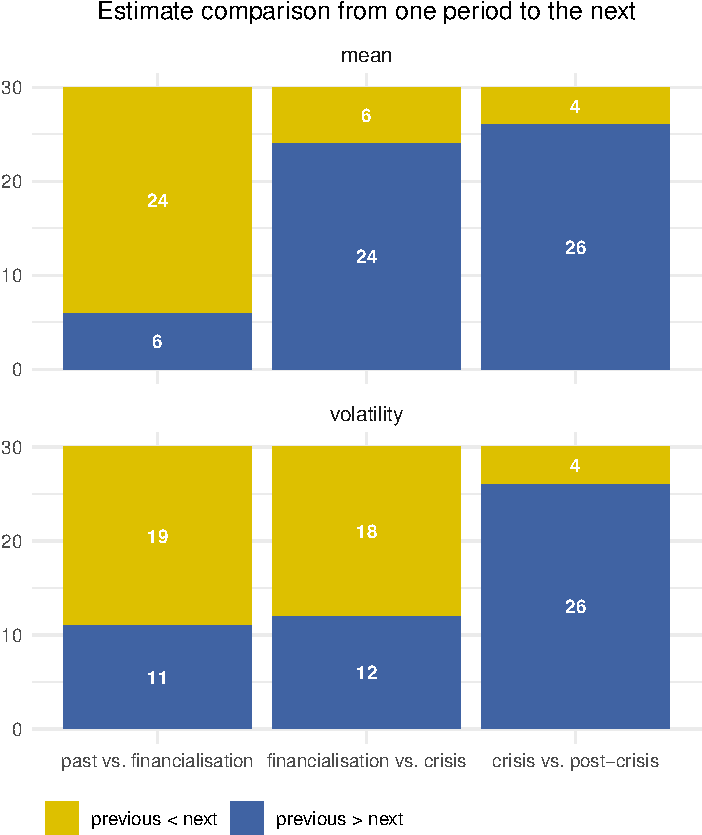
\includegraphics{paper_files/figure-pdf/fig-estimates-1.pdf}

}

\caption{\label{fig-estimates}This figure compares the evolution of
estimates for mean (top panel) and volatility (bottom panel) for
individual commodity returns across three period transitions: past →
financialisation, financialisation → crisis and crisis → post-crisis.
Each stacked bar shows how many cases fall into two categories: yellow
(the estimate in the previous period is smaller than in the next period)
and blue (the estimate in the previous period is larger than in the next
period); numbers inside the bars indicate the count of observations in
each category. Detailed results are available in the attached
\href{https://bautheac.shinyapps.io/co-movement/}{Internet Appendix}.
Period definitions are discussed in Section~\ref{sec-methods} while the
results are discussed in Section~\ref{sec-results}.}

\end{figure}%

\newpage

\begin{figure}

\centering{

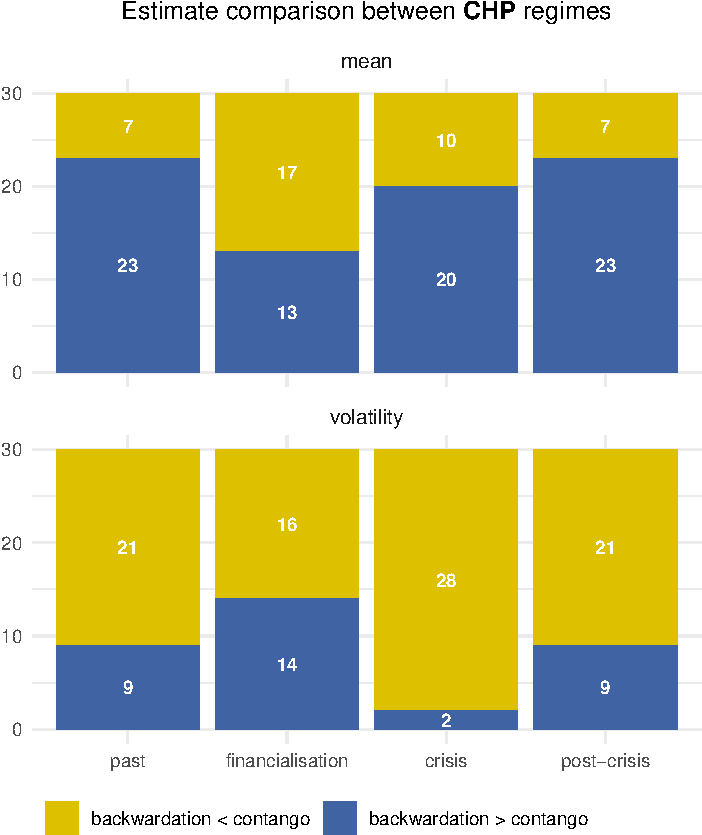
\includegraphics{paper_files/figure-pdf/fig-regimes-1.pdf}

}

\caption{\label{fig-regimes}This figure compares estimates for mean (top
panel) and volatility (bottom panel) for individual commodity returns
between \textbf{CHP} regime phases (\textbf{backwardation}
vs.~\textbf{contango}) for the four periods. Each stacked bar shows how
many cases fall into two categories: yellow (the estimate for the
\textbf{backwardation phase} is smaller than for the \textbf{contango}
phase) and blue (the estimate for the \textbf{backwardation phase} is
greater than for the \textbf{contango} phase); numbers inside the bars
indicate the count of observations in each category.
\textbf{Backwardation} and \textbf{contango} regimes as well as period
definitions are discussed in Section~\ref{sec-methods} while the results
are discussed in Section~\ref{sec-results}.}

\end{figure}%

\newpage

\section*{Tables}\label{tables}
\addcontentsline{toc}{section}{Tables}

\begingroup\fontsize{7}{9}\selectfont

\begin{longtable}[t]{>{}l>{}l>{}l>{}r>{}r>{}r>{}r}

\caption{\label{tbl-stats-regime-tests}This table shows mean returns and
volatilities for two equally weighted portfolios of US and GB traded
assets for the four periods. For each period, estimates are computed
independently over the whole period as well as over phases of
\textbf{backwardation} and \textbf{contango}. The table further shows
the results of t-tests of significance for the mean returns as well as
t-tests of difference between these when computed over the two phases
independently along with F-tests of difference for the corresponding
variances. Values significant at the 1\%, 5\% and 10\% level are marked
with ***, ** and * respectively. Detailed results are available in the
attached \href{https://bautheac.shinyapps.io/co-movement/}{Internet
Appendix}. \textbf{Backwardation} and \textbf{contango} regimes as well
as period definitions are discussed in Section~\ref{sec-methods} while
the results are discussed in Section~\ref{sec-results}.}

\tabularnewline

\toprule
\textcolor{black}{\textbf{asset}} & \textcolor{black}{\textbf{estimate}} & \textcolor{black}{\textbf{regime}} & \textcolor{black}{\textbf{past}} & \textcolor{black}{\textbf{financialisation}} & \textcolor{black}{\textbf{crisis}} & \textcolor{black}{\textbf{post-crisis}}\\
\midrule
\textbf{US commodities} & \textbf{mean} & \textbf{whole period} & \textcolor[HTML]{4285f4}{\textbf{*6.89\%}} & \textcolor[HTML]{4285f4}{\textbf{**15.89\%}} & \textcolor[HTML]{4285f4}{\textbf{9.39\%}} & \textcolor[HTML]{4285f4}{\textbf{-0.18\%}}\\
\textbf{} & \textbf{} & \textbf{backwardation} & \textcolor[HTML]{4285f4}{\textbf{***15.44\%}} & \textcolor[HTML]{4285f4}{\textbf{*15.66\%}} & \textcolor[HTML]{4285f4}{\textbf{13.4\%}} & \textcolor[HTML]{4285f4}{\textbf{6.82\%}}\\
\textbf{} & \textbf{} & \textbf{contango} & \textcolor[HTML]{4285f4}{\textbf{-1.09\%}} & \textcolor[HTML]{4285f4}{\textbf{*16.16\%}} & \textcolor[HTML]{4285f4}{\textbf{4.9\%}} & \textcolor[HTML]{4285f4}{\textbf{-6.33\%}}\\
\textbf{} & \textbf{} & \textbf{backwardation vs. contango} & \textcolor[HTML]{4285f4}{\textbf{**}} & \textcolor[HTML]{4285f4}{\textbf{}} & \textcolor[HTML]{4285f4}{\textbf{}} & \textcolor[HTML]{4285f4}{\textbf{}}\\
\textbf{} & \textbf{volatility} & \textbf{whole period} & \textcolor[HTML]{4285f4}{\textbf{10\%}} & \textcolor[HTML]{4285f4}{\textbf{13.62\%}} & \textcolor[HTML]{4285f4}{\textbf{17.58\%}} & \textcolor[HTML]{4285f4}{\textbf{9.86\%}}\\
\addlinespace
\textbf{} & \textbf{} & \textbf{backwardation} & \textcolor[HTML]{4285f4}{\textbf{9.88\%}} & \textcolor[HTML]{4285f4}{\textbf{14.21\%}} & \textcolor[HTML]{4285f4}{\textbf{14.83\%}} & \textcolor[HTML]{4285f4}{\textbf{8.59\%}}\\
\textbf{} & \textbf{} & \textbf{contango} & \textcolor[HTML]{4285f4}{\textbf{10.09\%}} & \textcolor[HTML]{4285f4}{\textbf{13.05\%}} & \textcolor[HTML]{4285f4}{\textbf{19.98\%}} & \textcolor[HTML]{4285f4}{\textbf{10.95\%}}\\
\textbf{} & \textbf{} & \textbf{backwardation vs. contango} & \textcolor[HTML]{4285f4}{\textbf{}} & \textcolor[HTML]{4285f4}{\textbf{**}} & \textcolor[HTML]{4285f4}{\textbf{***}} & \textcolor[HTML]{4285f4}{\textbf{***}}\\
\textbf{GB commodities} & \textbf{mean} & \textbf{whole period} & \textcolor[HTML]{4285f4}{\textbf{2.47\%}} & \textcolor[HTML]{4285f4}{\textbf{*21.77\%}} & \textcolor[HTML]{4285f4}{\textbf{5.25\%}} & \textcolor[HTML]{4285f4}{\textbf{2.72\%}}\\
\textbf{} & \textbf{} & \textbf{backwardation} & \textcolor[HTML]{4285f4}{\textbf{4.41\%}} & \textcolor[HTML]{4285f4}{\textbf{8.01\%}} & \textcolor[HTML]{4285f4}{\textbf{15.06\%}} & \textcolor[HTML]{4285f4}{\textbf{**19.95\%}}\\
\addlinespace
\textbf{} & \textbf{} & \textbf{contango} & \textcolor[HTML]{4285f4}{\textbf{0.34\%}} & \textcolor[HTML]{4285f4}{\textbf{*35.56\%}} & \textcolor[HTML]{4285f4}{\textbf{-5.24\%}} & \textcolor[HTML]{4285f4}{\textbf{-14.05\%}}\\
\textbf{} & \textbf{} & \textbf{backwardation vs. contango} & \textcolor[HTML]{4285f4}{\textbf{}} & \textcolor[HTML]{4285f4}{\textbf{}} & \textcolor[HTML]{4285f4}{\textbf{}} & \textcolor[HTML]{4285f4}{\textbf{**}}\\
\textbf{} & \textbf{volatility} & \textbf{whole period} & \textcolor[HTML]{4285f4}{\textbf{15.66\%}} & \textcolor[HTML]{4285f4}{\textbf{26.91\%}} & \textcolor[HTML]{4285f4}{\textbf{30.24\%}} & \textcolor[HTML]{4285f4}{\textbf{16.19\%}}\\
\textbf{} & \textbf{} & \textbf{backwardation} & \textcolor[HTML]{4285f4}{\textbf{14.39\%}} & \textcolor[HTML]{4285f4}{\textbf{25.92\%}} & \textcolor[HTML]{4285f4}{\textbf{25.94\%}} & \textcolor[HTML]{4285f4}{\textbf{15.13\%}}\\
\textbf{} & \textbf{} & \textbf{contango} & \textcolor[HTML]{4285f4}{\textbf{16.87\%}} & \textcolor[HTML]{4285f4}{\textbf{27.88\%}} & \textcolor[HTML]{4285f4}{\textbf{34.06\%}} & \textcolor[HTML]{4285f4}{\textbf{17.1\%}}\\
\addlinespace
\textbf{} & \textbf{} & \textbf{backwardation vs. contango} & \textcolor[HTML]{4285f4}{\textbf{***}} & \textcolor[HTML]{4285f4}{\textbf{*}} & \textcolor[HTML]{4285f4}{\textbf{***}} & \textcolor[HTML]{4285f4}{\textbf{***}}\\
\bottomrule

\end{longtable}

\endgroup{}

\newpage

\begingroup\fontsize{7}{9}\selectfont

\begin{longtable}[t]{>{}l>{}l>{}l>{}r>{}r>{}r>{}r}

\caption{\label{tbl-time-reg-US-CHP}This table shows the average time
series \(R^{2}\) for models where the returns series for the individual
US traded commodities are independently regressed against relative
change in their own commercial hedging pressure (CHP) series as well as
against that in \textbf{CHP}, a market wide measure of CHP which
calculation method is discussed in Section~\ref{sec-methods}. Averages
are computed independently across the whole cross-section of US traded
commodity assets as well as across commodity sectors and sub-sectors for
the four periods. Period definitions are discussed in
Section~\ref{sec-methods} while the results are discussed in
Section~\ref{sec-results} and the commodity assets taxonomy is detailed
in Section~\ref{sec-taxonomy}.}

\tabularnewline

\toprule
\textcolor{black}{\textbf{regressor}} & \textcolor{black}{\textbf{sector}} & \textcolor{black}{\textbf{sub-sector}} & \textcolor{black}{\textbf{past}} & \textcolor{black}{\textbf{financialisation}} & \textcolor{black}{\textbf{crisis}} & \textcolor{black}{\textbf{post-crisis}}\\
\midrule
\textbf{Δ\% commodity CHP} & \textbf{all} & \textbf{all} & \textcolor[HTML]{4285f4}{\textbf{25.79\%}} & \textcolor[HTML]{4285f4}{\textbf{20.72\%}} & \textcolor[HTML]{4285f4}{\textbf{22.46\%}} & \textcolor[HTML]{4285f4}{\textbf{27.17\%}}\\
\textbf{} & \textbf{agriculturals} & \textbf{all} & \textcolor[HTML]{4285f4}{\textbf{25.19\%}} & \textcolor[HTML]{4285f4}{\textbf{21.6\%}} & \textcolor[HTML]{4285f4}{\textbf{23.91\%}} & \textcolor[HTML]{4285f4}{\textbf{28.12\%}}\\
\textbf{} & \textbf{} & \textbf{grains} & \textcolor[HTML]{4285f4}{\textbf{33.18\%}} & \textcolor[HTML]{4285f4}{\textbf{27.86\%}} & \textcolor[HTML]{4285f4}{\textbf{29.15\%}} & \textcolor[HTML]{4285f4}{\textbf{36.24\%}}\\
\textbf{} & \textbf{} & \textbf{livestock} & \textcolor[HTML]{4285f4}{\textbf{6.23\%}} & \textcolor[HTML]{4285f4}{\textbf{10.53\%}} & \textcolor[HTML]{4285f4}{\textbf{6.89\%}} & \textcolor[HTML]{4285f4}{\textbf{4.34\%}}\\
\textbf{} & \textbf{} & \textbf{softs} & \textcolor[HTML]{4285f4}{\textbf{26.68\%}} & \textcolor[HTML]{4285f4}{\textbf{20.89\%}} & \textcolor[HTML]{4285f4}{\textbf{27.19\%}} & \textcolor[HTML]{4285f4}{\textbf{31.88\%}}\\
\addlinespace
\textbf{} & \textbf{energy} & \textbf{all} & \textcolor[HTML]{4285f4}{\textbf{25.12\%}} & \textcolor[HTML]{4285f4}{\textbf{19.45\%}} & \textcolor[HTML]{4285f4}{\textbf{16\%}} & \textcolor[HTML]{4285f4}{\textbf{10.96\%}}\\
\textbf{} & \textbf{} & \textbf{gas} & \textcolor[HTML]{4285f4}{\textbf{19.69\%}} & \textcolor[HTML]{4285f4}{\textbf{15.65\%}} & \textcolor[HTML]{4285f4}{\textbf{7.36\%}} & \textcolor[HTML]{4285f4}{\textbf{5.29\%}}\\
\textbf{} & \textbf{} & \textbf{petroleum} & \textcolor[HTML]{4285f4}{\textbf{26.93\%}} & \textcolor[HTML]{4285f4}{\textbf{20.71\%}} & \textcolor[HTML]{4285f4}{\textbf{18.87\%}} & \textcolor[HTML]{4285f4}{\textbf{12.85\%}}\\
\textbf{} & \textbf{metals} & \textbf{all} & \textcolor[HTML]{4285f4}{\textbf{28.12\%}} & \textcolor[HTML]{4285f4}{\textbf{19.1\%}} & \textcolor[HTML]{4285f4}{\textbf{23.27\%}} & \textcolor[HTML]{4285f4}{\textbf{37.32\%}}\\
\textbf{} & \textbf{} & \textbf{base} & \textcolor[HTML]{4285f4}{\textbf{47.38\%}} & \textcolor[HTML]{4285f4}{\textbf{25.86\%}} & \textcolor[HTML]{4285f4}{\textbf{18.07\%}} & \textcolor[HTML]{4285f4}{\textbf{34.9\%}}\\
\addlinespace
\textbf{} & \textbf{} & \textbf{precious} & \textcolor[HTML]{4285f4}{\textbf{23.3\%}} & \textcolor[HTML]{4285f4}{\textbf{17.41\%}} & \textcolor[HTML]{4285f4}{\textbf{24.57\%}} & \textcolor[HTML]{4285f4}{\textbf{37.93\%}}\\
\textbf{Δ\% aggregate CHP} & \textbf{all} & \textbf{all} & \textcolor[HTML]{4285f4}{\textbf{5.37\%}} & \textcolor[HTML]{4285f4}{\textbf{7.12\%}} & \textcolor[HTML]{4285f4}{\textbf{14.72\%}} & \textcolor[HTML]{4285f4}{\textbf{7.49\%}}\\
\textbf{} & \textbf{agriculturals} & \textbf{all} & \textcolor[HTML]{4285f4}{\textbf{4.91\%}} & \textcolor[HTML]{4285f4}{\textbf{4.5\%}} & \textcolor[HTML]{4285f4}{\textbf{12.14\%}} & \textcolor[HTML]{4285f4}{\textbf{6.23\%}}\\
\textbf{} & \textbf{} & \textbf{grains} & \textcolor[HTML]{4285f4}{\textbf{7.25\%}} & \textcolor[HTML]{4285f4}{\textbf{5.4\%}} & \textcolor[HTML]{4285f4}{\textbf{19.75\%}} & \textcolor[HTML]{4285f4}{\textbf{8.45\%}}\\
\textbf{} & \textbf{} & \textbf{livestock} & \textcolor[HTML]{4285f4}{\textbf{1.35\%}} & \textcolor[HTML]{4285f4}{\textbf{0.41\%}} & \textcolor[HTML]{4285f4}{\textbf{0.52\%}} & \textcolor[HTML]{4285f4}{\textbf{0.26\%}}\\
\addlinespace
\textbf{} & \textbf{} & \textbf{softs} & \textcolor[HTML]{4285f4}{\textbf{4.34\%}} & \textcolor[HTML]{4285f4}{\textbf{5.64\%}} & \textcolor[HTML]{4285f4}{\textbf{10.35\%}} & \textcolor[HTML]{4285f4}{\textbf{6.98\%}}\\
\textbf{} & \textbf{energy} & \textbf{all} & \textcolor[HTML]{4285f4}{\textbf{3.35\%}} & \textcolor[HTML]{4285f4}{\textbf{6.27\%}} & \textcolor[HTML]{4285f4}{\textbf{14.83\%}} & \textcolor[HTML]{4285f4}{\textbf{2.45\%}}\\
\textbf{} & \textbf{} & \textbf{gas} & \textcolor[HTML]{4285f4}{\textbf{2.65\%}} & \textcolor[HTML]{4285f4}{\textbf{2.58\%}} & \textcolor[HTML]{4285f4}{\textbf{2.6\%}} & \textcolor[HTML]{4285f4}{\textbf{0.27\%}}\\
\textbf{} & \textbf{} & \textbf{petroleum} & \textcolor[HTML]{4285f4}{\textbf{3.59\%}} & \textcolor[HTML]{4285f4}{\textbf{7.49\%}} & \textcolor[HTML]{4285f4}{\textbf{18.9\%}} & \textcolor[HTML]{4285f4}{\textbf{3.17\%}}\\
\textbf{} & \textbf{metals} & \textbf{all} & \textcolor[HTML]{4285f4}{\textbf{8.36\%}} & \textcolor[HTML]{4285f4}{\textbf{15.67\%}} & \textcolor[HTML]{4285f4}{\textbf{22.37\%}} & \textcolor[HTML]{4285f4}{\textbf{15.33\%}}\\
\addlinespace
\textbf{} & \textbf{} & \textbf{base} & \textcolor[HTML]{4285f4}{\textbf{10.12\%}} & \textcolor[HTML]{4285f4}{\textbf{12.74\%}} & \textcolor[HTML]{4285f4}{\textbf{23.94\%}} & \textcolor[HTML]{4285f4}{\textbf{7.67\%}}\\
\textbf{} & \textbf{} & \textbf{precious} & \textcolor[HTML]{4285f4}{\textbf{7.92\%}} & \textcolor[HTML]{4285f4}{\textbf{16.4\%}} & \textcolor[HTML]{4285f4}{\textbf{21.98\%}} & \textcolor[HTML]{4285f4}{\textbf{17.25\%}}\\
\bottomrule

\end{longtable}

\endgroup{}

\newpage

\begingroup\fontsize{7}{9}\selectfont

\begin{longtable}[t]{>{}l>{}l>{}l>{}r>{}r>{}r>{}r>{}r}

\caption{\label{tbl-correlations-inner-periods}This table shows the
average return pairwise correlation coefficients computed independently
across the whole cross-section of individual commodity assets as well as
within countries and commodity sectors and sub-sectors for the four
periods. For each period, the results are computed independently over
the entire period as well as over phases of \textbf{backwardation} and
\textbf{contango}. \textbf{Backwardation} and \textbf{contango} regimes
as well as period definitions are discussed in Section~\ref{sec-methods}
while the results are discussed in Section~\ref{sec-results} and the
commodity assets taxonomy is detailed in Section~\ref{sec-taxonomy}.}

\tabularnewline

\toprule
\textcolor{black}{\textbf{country}} & \textcolor{black}{\textbf{sector}} & \textcolor{black}{\textbf{sub-sector}} & \textcolor{black}{\textbf{regime}} & \textcolor{black}{\textbf{past}} & \textcolor{black}{\textbf{financialisation}} & \textcolor{black}{\textbf{crisis}} & \textcolor{black}{\textbf{post-crisis}}\\
\midrule
\textbf{all} & \textbf{all} & \textbf{all} & \textbf{whole period} & \textcolor[HTML]{4285f4}{\textbf{0.0737}} & \textcolor[HTML]{4285f4}{\textbf{0.1638}} & \textcolor[HTML]{4285f4}{\textbf{0.2849}} & \textcolor[HTML]{4285f4}{\textbf{0.1282}}\\
\textbf{} & \textbf{} & \textbf{} & \textbf{backwardation} & \textcolor[HTML]{4285f4}{\textbf{0.0724}} & \textcolor[HTML]{4285f4}{\textbf{0.1790}} & \textcolor[HTML]{4285f4}{\textbf{0.2709}} & \textcolor[HTML]{4285f4}{\textbf{0.1001}}\\
\textbf{} & \textbf{} & \textbf{} & \textbf{contango} & \textcolor[HTML]{4285f4}{\textbf{0.0748}} & \textcolor[HTML]{4285f4}{\textbf{0.1501}} & \textcolor[HTML]{4285f4}{\textbf{0.2985}} & \textcolor[HTML]{4285f4}{\textbf{0.1495}}\\
\textbf{US} & \textbf{all} & \textbf{all} & \textbf{whole period} & \textcolor[HTML]{4285f4}{\textbf{0.0684}} & \textcolor[HTML]{4285f4}{\textbf{0.1545}} & \textcolor[HTML]{4285f4}{\textbf{0.2526}} & \textcolor[HTML]{4285f4}{\textbf{0.1096}}\\
\textbf{} & \textbf{} & \textbf{} & \textbf{backwardation} & \textcolor[HTML]{4285f4}{\textbf{0.0642}} & \textcolor[HTML]{4285f4}{\textbf{0.1697}} & \textcolor[HTML]{4285f4}{\textbf{0.2323}} & \textcolor[HTML]{4285f4}{\textbf{0.0859}}\\
\addlinespace
\textbf{} & \textbf{} & \textbf{} & \textbf{contango} & \textcolor[HTML]{4285f4}{\textbf{0.0720}} & \textcolor[HTML]{4285f4}{\textbf{0.1402}} & \textcolor[HTML]{4285f4}{\textbf{0.2706}} & \textcolor[HTML]{4285f4}{\textbf{0.1268}}\\
\textbf{} & \textbf{agriculturals} & \textbf{all} & \textbf{whole period} & \textcolor[HTML]{4285f4}{\textbf{0.0910}} & \textcolor[HTML]{4285f4}{\textbf{0.1305}} & \textcolor[HTML]{4285f4}{\textbf{0.2322}} & \textcolor[HTML]{4285f4}{\textbf{0.1075}}\\
\textbf{} & \textbf{} & \textbf{} & \textbf{backwardation} & \textcolor[HTML]{4285f4}{\textbf{0.0799}} & \textcolor[HTML]{4285f4}{\textbf{0.1421}} & \textcolor[HTML]{4285f4}{\textbf{0.1975}} & \textcolor[HTML]{4285f4}{\textbf{0.0955}}\\
\textbf{} & \textbf{} & \textbf{} & \textbf{contango} & \textcolor[HTML]{4285f4}{\textbf{0.1018}} & \textcolor[HTML]{4285f4}{\textbf{0.1184}} & \textcolor[HTML]{4285f4}{\textbf{0.2611}} & \textcolor[HTML]{4285f4}{\textbf{0.1186}}\\
\textbf{} & \textbf{} & \textbf{grains} & \textbf{whole period} & \textcolor[HTML]{4285f4}{\textbf{0.4421}} & \textcolor[HTML]{4285f4}{\textbf{0.4898}} & \textcolor[HTML]{4285f4}{\textbf{0.5673}} & \textcolor[HTML]{4285f4}{\textbf{0.3728}}\\
\addlinespace
\textbf{} & \textbf{} & \textbf{} & \textbf{backwardation} & \textcolor[HTML]{4285f4}{\textbf{0.4312}} & \textcolor[HTML]{4285f4}{\textbf{0.5283}} & \textcolor[HTML]{4285f4}{\textbf{0.5749}} & \textcolor[HTML]{4285f4}{\textbf{0.3289}}\\
\textbf{} & \textbf{} & \textbf{} & \textbf{contango} & \textcolor[HTML]{4285f4}{\textbf{0.4570}} & \textcolor[HTML]{4285f4}{\textbf{0.4510}} & \textcolor[HTML]{4285f4}{\textbf{0.5675}} & \textcolor[HTML]{4285f4}{\textbf{0.4161}}\\
\textbf{} & \textbf{} & \textbf{livestock} & \textbf{whole period} & \textcolor[HTML]{4285f4}{\textbf{0.3340}} & \textcolor[HTML]{4285f4}{\textbf{0.2868}} & \textcolor[HTML]{4285f4}{\textbf{0.3707}} & \textcolor[HTML]{4285f4}{\textbf{0.3333}}\\
\textbf{} & \textbf{} & \textbf{} & \textbf{backwardation} & \textcolor[HTML]{4285f4}{\textbf{0.3053}} & \textcolor[HTML]{4285f4}{\textbf{0.2652}} & \textcolor[HTML]{4285f4}{\textbf{0.3906}} & \textcolor[HTML]{4285f4}{\textbf{0.3220}}\\
\textbf{} & \textbf{} & \textbf{} & \textbf{contango} & \textcolor[HTML]{4285f4}{\textbf{0.3605}} & \textcolor[HTML]{4285f4}{\textbf{0.3150}} & \textcolor[HTML]{4285f4}{\textbf{0.3557}} & \textcolor[HTML]{4285f4}{\textbf{0.3483}}\\
\addlinespace
\textbf{} & \textbf{} & \textbf{softs} & \textbf{whole period} & \textcolor[HTML]{4285f4}{\textbf{0.0391}} & \textcolor[HTML]{4285f4}{\textbf{0.0853}} & \textcolor[HTML]{4285f4}{\textbf{0.1584}} & \textcolor[HTML]{4285f4}{\textbf{0.0764}}\\
\textbf{} & \textbf{} & \textbf{} & \textbf{backwardation} & \textcolor[HTML]{4285f4}{\textbf{0.0437}} & \textcolor[HTML]{4285f4}{\textbf{0.0845}} & \textcolor[HTML]{4285f4}{\textbf{0.1210}} & \textcolor[HTML]{4285f4}{\textbf{0.0685}}\\
\textbf{} & \textbf{} & \textbf{} & \textbf{contango} & \textcolor[HTML]{4285f4}{\textbf{0.0334}} & \textcolor[HTML]{4285f4}{\textbf{0.0874}} & \textcolor[HTML]{4285f4}{\textbf{0.1937}} & \textcolor[HTML]{4285f4}{\textbf{0.0833}}\\
\textbf{} & \textbf{energy} & \textbf{all} & \textbf{whole period} & \textcolor[HTML]{4285f4}{\textbf{0.4908}} & \textcolor[HTML]{4285f4}{\textbf{0.5892}} & \textcolor[HTML]{4285f4}{\textbf{0.4687}} & \textcolor[HTML]{4285f4}{\textbf{0.4203}}\\
\textbf{} & \textbf{} & \textbf{} & \textbf{backwardation} & \textcolor[HTML]{4285f4}{\textbf{0.4844}} & \textcolor[HTML]{4285f4}{\textbf{0.5949}} & \textcolor[HTML]{4285f4}{\textbf{0.4601}} & \textcolor[HTML]{4285f4}{\textbf{0.4179}}\\
\addlinespace
\textbf{} & \textbf{} & \textbf{} & \textbf{contango} & \textcolor[HTML]{4285f4}{\textbf{0.4957}} & \textcolor[HTML]{4285f4}{\textbf{0.5869}} & \textcolor[HTML]{4285f4}{\textbf{0.4779}} & \textcolor[HTML]{4285f4}{\textbf{0.4210}}\\
\textbf{} & \textbf{} & \textbf{petroleum} & \textbf{whole period} & \textcolor[HTML]{4285f4}{\textbf{0.7278}} & \textcolor[HTML]{4285f4}{\textbf{0.7846}} & \textcolor[HTML]{4285f4}{\textbf{0.7692}} & \textcolor[HTML]{4285f4}{\textbf{0.7175}}\\
\textbf{} & \textbf{} & \textbf{} & \textbf{backwardation} & \textcolor[HTML]{4285f4}{\textbf{0.6962}} & \textcolor[HTML]{4285f4}{\textbf{0.7854}} & \textcolor[HTML]{4285f4}{\textbf{0.7727}} & \textcolor[HTML]{4285f4}{\textbf{0.7282}}\\
\textbf{} & \textbf{} & \textbf{} & \textbf{contango} & \textcolor[HTML]{4285f4}{\textbf{0.7606}} & \textcolor[HTML]{4285f4}{\textbf{0.7856}} & \textcolor[HTML]{4285f4}{\textbf{0.7716}} & \textcolor[HTML]{4285f4}{\textbf{0.7134}}\\
\textbf{} & \textbf{metals} & \textbf{all} & \textbf{whole period} & \textcolor[HTML]{4285f4}{\textbf{0.2167}} & \textcolor[HTML]{4285f4}{\textbf{0.5553}} & \textcolor[HTML]{4285f4}{\textbf{0.5877}} & \textcolor[HTML]{4285f4}{\textbf{0.4721}}\\
\addlinespace
\textbf{} & \textbf{} & \textbf{} & \textbf{backwardation} & \textcolor[HTML]{4285f4}{\textbf{0.2201}} & \textcolor[HTML]{4285f4}{\textbf{0.5418}} & \textcolor[HTML]{4285f4}{\textbf{0.6353}} & \textcolor[HTML]{4285f4}{\textbf{0.4155}}\\
\textbf{} & \textbf{} & \textbf{} & \textbf{contango} & \textcolor[HTML]{4285f4}{\textbf{0.2145}} & \textcolor[HTML]{4285f4}{\textbf{0.5727}} & \textcolor[HTML]{4285f4}{\textbf{0.5709}} & \textcolor[HTML]{4285f4}{\textbf{0.5035}}\\
\textbf{} & \textbf{} & \textbf{precious} & \textbf{whole period} & \textcolor[HTML]{4285f4}{\textbf{0.2883}} & \textcolor[HTML]{4285f4}{\textbf{0.6305}} & \textcolor[HTML]{4285f4}{\textbf{0.6704}} & \textcolor[HTML]{4285f4}{\textbf{0.5762}}\\
\textbf{} & \textbf{} & \textbf{} & \textbf{backwardation} & \textcolor[HTML]{4285f4}{\textbf{0.3070}} & \textcolor[HTML]{4285f4}{\textbf{0.6061}} & \textcolor[HTML]{4285f4}{\textbf{0.6991}} & \textcolor[HTML]{4285f4}{\textbf{0.5386}}\\
\textbf{} & \textbf{} & \textbf{} & \textbf{contango} & \textcolor[HTML]{4285f4}{\textbf{0.2713}} & \textcolor[HTML]{4285f4}{\textbf{0.6591}} & \textcolor[HTML]{4285f4}{\textbf{0.6615}} & \textcolor[HTML]{4285f4}{\textbf{0.5949}}\\
\addlinespace
\textbf{GB} & \textbf{all} & \textbf{all} & \textbf{whole period} & \textcolor[HTML]{4285f4}{\textbf{0.4047}} & \textcolor[HTML]{4285f4}{\textbf{0.4691}} & \textcolor[HTML]{4285f4}{\textbf{0.6536}} & \textcolor[HTML]{4285f4}{\textbf{0.4412}}\\
\textbf{} & \textbf{} & \textbf{} & \textbf{backwardation} & \textcolor[HTML]{4285f4}{\textbf{0.3987}} & \textcolor[HTML]{4285f4}{\textbf{0.4753}} & \textcolor[HTML]{4285f4}{\textbf{0.6729}} & \textcolor[HTML]{4285f4}{\textbf{0.3954}}\\
\textbf{} & \textbf{} & \textbf{} & \textbf{contango} & \textcolor[HTML]{4285f4}{\textbf{0.4108}} & \textcolor[HTML]{4285f4}{\textbf{0.4652}} & \textcolor[HTML]{4285f4}{\textbf{0.6456}} & \textcolor[HTML]{4285f4}{\textbf{0.4797}}\\
\bottomrule

\end{longtable}

\endgroup{}

\newpage

\begingroup\fontsize{7}{9}\selectfont

\begin{longtable}[t]{>{}l>{}r>{}r>{}r>{}r}

\caption{\label{tbl-correlations-cross-periods}This table shows the
average return pairwise correlation coefficients between equally
weighted US sub-sector portfolios (agriculturals: gains, livestock,
softs; energy: gas, petroleum; metals: base, precious) independently
computed for the four periods. For each period, the results are further
computed independently over the entire period as well as over phases
\textbf{backwardation} and \textbf{contango}. \textbf{Backwardation} and
\textbf{contango} regimes as well as period definitions are discussed in
Section~\ref{sec-methods} while the results are discussed in
Section~\ref{sec-results} and the commodity assets taxonomy is detailed
in Section~\ref{sec-taxonomy}.}

\tabularnewline

\toprule
\textcolor{black}{\textbf{regime}} & \textcolor{black}{\textbf{past}} & \textcolor{black}{\textbf{financialisation}} & \textcolor{black}{\textbf{crisis}} & \textcolor{black}{\textbf{post-crisis}}\\
\midrule
\textbf{whole period} & \textcolor[HTML]{4285f4}{\textbf{0.0421}} & \textcolor[HTML]{4285f4}{\textbf{0.0631}} & \textcolor[HTML]{4285f4}{\textbf{0.0799}} & \textcolor[HTML]{4285f4}{\textbf{0.0778}}\\
\textbf{backwardation} & \textcolor[HTML]{4285f4}{\textbf{0.1166}} & \textcolor[HTML]{4285f4}{\textbf{0.0201}} & \textcolor[HTML]{4285f4}{\textbf{0.0633}} & \textcolor[HTML]{4285f4}{\textbf{0.0727}}\\
\textbf{contango} & \textcolor[HTML]{4285f4}{\textbf{0.0297}} & \textcolor[HTML]{4285f4}{\textbf{0.1164}} & \textcolor[HTML]{4285f4}{\textbf{0.0889}} & \textcolor[HTML]{4285f4}{\textbf{0.0812}}\\
\bottomrule

\end{longtable}

\endgroup{}

\newpage

\begin{landscape}\begingroup\fontsize{7}{9}\selectfont

\begin{longtable}[t]{>{}l>{}l>{}l>{}l>{}r>{}r>{}r>{}r>{}r>{}r>{}r>{}r>{}r>{}r}

\caption{\label{tbl-correlations-inner-years}While
Table~\ref{tbl-correlations-inner-periods} shows results computed
independently for the four periods, this table shows the results of the
same analysis implemented for each year over the entire sample period.
The results are discussed in Section~\ref{sec-results} while
Section~\ref{sec-taxonomy} details the commodity assets taxonomy.}

\tabularnewline

\toprule
\textcolor{black}{\textbf{country}} & \textcolor{black}{\textbf{sector}} & \textcolor{black}{\textbf{sub-sector}} & \textcolor{black}{\textbf{decade}} & \textcolor{black}{\textbf{0}} & \textcolor{black}{\textbf{1}} & \textcolor{black}{\textbf{2}} & \textcolor{black}{\textbf{3}} & \textcolor{black}{\textbf{4}} & \textcolor{black}{\textbf{5}} & \textcolor{black}{\textbf{6}} & \textcolor{black}{\textbf{7}} & \textcolor{black}{\textbf{8}} & \textcolor{black}{\textbf{9}}\\
\midrule
\textbf{all} & \textbf{all} & \textbf{all} & \textbf{1990} & \textcolor[HTML]{4285f4}{\textbf{}} & \textcolor[HTML]{4285f4}{\textbf{}} & \textcolor[HTML]{4285f4}{\textbf{}} & \textcolor[HTML]{4285f4}{\textbf{}} & \textcolor[HTML]{4285f4}{\textbf{}} & \textcolor[HTML]{4285f4}{\textbf{}} & \textcolor[HTML]{4285f4}{\textbf{}} & \textcolor[HTML]{4285f4}{\textbf{0.0401}} & \textcolor[HTML]{4285f4}{\textbf{0.0812}} & \textcolor[HTML]{4285f4}{\textbf{0.0822}}\\
\textbf{} & \textbf{} & \textbf{} & \textbf{2000} & \textcolor[HTML]{4285f4}{\textbf{0.0652}} & \textcolor[HTML]{4285f4}{\textbf{0.0719}} & \textcolor[HTML]{4285f4}{\textbf{0.0796}} & \textcolor[HTML]{4285f4}{\textbf{0.0848}} & \textcolor[HTML]{4285f4}{\textbf{0.1242}} & \textcolor[HTML]{4285f4}{\textbf{0.1247}} & \textcolor[HTML]{4285f4}{\textbf{0.1650}} & \textcolor[HTML]{4285f4}{\textbf{0.1541}} & \textcolor[HTML]{4285f4}{\textbf{0.3334}} & \textcolor[HTML]{4285f4}{\textbf{0.2913}}\\
\textbf{} & \textbf{} & \textbf{} & \textbf{2010} & \textcolor[HTML]{4285f4}{\textbf{0.2743}} & \textcolor[HTML]{4285f4}{\textbf{0.2837}} & \textcolor[HTML]{4285f4}{\textbf{0.2235}} & \textcolor[HTML]{4285f4}{\textbf{0.1432}} & \textcolor[HTML]{4285f4}{\textbf{0.1139}} & \textcolor[HTML]{4285f4}{\textbf{0.1547}} & \textcolor[HTML]{4285f4}{\textbf{0.1339}} & \textcolor[HTML]{4285f4}{\textbf{0.0963}} & \textcolor[HTML]{4285f4}{\textbf{0.1374}} & \textcolor[HTML]{4285f4}{\textbf{}}\\
\textbf{US} & \textbf{all} & \textbf{all} & \textbf{1990} & \textcolor[HTML]{4285f4}{\textbf{}} & \textcolor[HTML]{4285f4}{\textbf{}} & \textcolor[HTML]{4285f4}{\textbf{}} & \textcolor[HTML]{4285f4}{\textbf{}} & \textcolor[HTML]{4285f4}{\textbf{}} & \textcolor[HTML]{4285f4}{\textbf{}} & \textcolor[HTML]{4285f4}{\textbf{}} & \textcolor[HTML]{4285f4}{\textbf{0.0536}} & \textcolor[HTML]{4285f4}{\textbf{0.0811}} & \textcolor[HTML]{4285f4}{\textbf{0.0803}}\\
\textbf{} & \textbf{} & \textbf{} & \textbf{2000} & \textcolor[HTML]{4285f4}{\textbf{0.0597}} & \textcolor[HTML]{4285f4}{\textbf{0.0652}} & \textcolor[HTML]{4285f4}{\textbf{0.0600}} & \textcolor[HTML]{4285f4}{\textbf{0.0723}} & \textcolor[HTML]{4285f4}{\textbf{0.1073}} & \textcolor[HTML]{4285f4}{\textbf{0.1164}} & \textcolor[HTML]{4285f4}{\textbf{0.1502}} & \textcolor[HTML]{4285f4}{\textbf{0.1479}} & \textcolor[HTML]{4285f4}{\textbf{0.3284}} & \textcolor[HTML]{4285f4}{\textbf{0.2621}}\\
\addlinespace
\textbf{} & \textbf{} & \textbf{} & \textbf{2010} & \textcolor[HTML]{4285f4}{\textbf{0.2275}} & \textcolor[HTML]{4285f4}{\textbf{0.2541}} & \textcolor[HTML]{4285f4}{\textbf{0.1850}} & \textcolor[HTML]{4285f4}{\textbf{0.1018}} & \textcolor[HTML]{4285f4}{\textbf{0.0986}} & \textcolor[HTML]{4285f4}{\textbf{0.1371}} & \textcolor[HTML]{4285f4}{\textbf{0.1064}} & \textcolor[HTML]{4285f4}{\textbf{0.0905}} & \textcolor[HTML]{4285f4}{\textbf{0.1197}} & \textcolor[HTML]{4285f4}{\textbf{}}\\
\textbf{} & \textbf{agriculturals} & \textbf{all} & \textbf{1990} & \textcolor[HTML]{4285f4}{\textbf{}} & \textcolor[HTML]{4285f4}{\textbf{}} & \textcolor[HTML]{4285f4}{\textbf{}} & \textcolor[HTML]{4285f4}{\textbf{}} & \textcolor[HTML]{4285f4}{\textbf{}} & \textcolor[HTML]{4285f4}{\textbf{}} & \textcolor[HTML]{4285f4}{\textbf{}} & \textcolor[HTML]{4285f4}{\textbf{0.0827}} & \textcolor[HTML]{4285f4}{\textbf{0.0916}} & \textcolor[HTML]{4285f4}{\textbf{0.1121}}\\
\textbf{} & \textbf{} & \textbf{} & \textbf{2000} & \textcolor[HTML]{4285f4}{\textbf{0.0918}} & \textcolor[HTML]{4285f4}{\textbf{0.0967}} & \textcolor[HTML]{4285f4}{\textbf{0.0734}} & \textcolor[HTML]{4285f4}{\textbf{0.0827}} & \textcolor[HTML]{4285f4}{\textbf{0.1111}} & \textcolor[HTML]{4285f4}{\textbf{0.1090}} & \textcolor[HTML]{4285f4}{\textbf{0.1125}} & \textcolor[HTML]{4285f4}{\textbf{0.1131}} & \textcolor[HTML]{4285f4}{\textbf{0.3034}} & \textcolor[HTML]{4285f4}{\textbf{0.2507}}\\
\textbf{} & \textbf{} & \textbf{} & \textbf{2010} & \textcolor[HTML]{4285f4}{\textbf{0.2038}} & \textcolor[HTML]{4285f4}{\textbf{0.2304}} & \textcolor[HTML]{4285f4}{\textbf{0.1583}} & \textcolor[HTML]{4285f4}{\textbf{0.0716}} & \textcolor[HTML]{4285f4}{\textbf{0.0846}} & \textcolor[HTML]{4285f4}{\textbf{0.1360}} & \textcolor[HTML]{4285f4}{\textbf{0.1121}} & \textcolor[HTML]{4285f4}{\textbf{0.1148}} & \textcolor[HTML]{4285f4}{\textbf{0.1181}} & \textcolor[HTML]{4285f4}{\textbf{}}\\
\textbf{} & \textbf{} & \textbf{grains} & \textbf{1990} & \textcolor[HTML]{4285f4}{\textbf{}} & \textcolor[HTML]{4285f4}{\textbf{}} & \textcolor[HTML]{4285f4}{\textbf{}} & \textcolor[HTML]{4285f4}{\textbf{}} & \textcolor[HTML]{4285f4}{\textbf{}} & \textcolor[HTML]{4285f4}{\textbf{}} & \textcolor[HTML]{4285f4}{\textbf{}} & \textcolor[HTML]{4285f4}{\textbf{0.5243}} & \textcolor[HTML]{4285f4}{\textbf{0.4882}} & \textcolor[HTML]{4285f4}{\textbf{0.5650}}\\
\addlinespace
\textbf{} & \textbf{} & \textbf{} & \textbf{2000} & \textcolor[HTML]{4285f4}{\textbf{0.4870}} & \textcolor[HTML]{4285f4}{\textbf{0.4337}} & \textcolor[HTML]{4285f4}{\textbf{0.3851}} & \textcolor[HTML]{4285f4}{\textbf{0.3402}} & \textcolor[HTML]{4285f4}{\textbf{0.4473}} & \textcolor[HTML]{4285f4}{\textbf{0.5335}} & \textcolor[HTML]{4285f4}{\textbf{0.4594}} & \textcolor[HTML]{4285f4}{\textbf{0.5040}} & \textcolor[HTML]{4285f4}{\textbf{0.6325}} & \textcolor[HTML]{4285f4}{\textbf{0.5681}}\\
\textbf{} & \textbf{} & \textbf{} & \textbf{2010} & \textcolor[HTML]{4285f4}{\textbf{0.5389}} & \textcolor[HTML]{4285f4}{\textbf{0.6424}} & \textcolor[HTML]{4285f4}{\textbf{0.5592}} & \textcolor[HTML]{4285f4}{\textbf{0.3199}} & \textcolor[HTML]{4285f4}{\textbf{0.3134}} & \textcolor[HTML]{4285f4}{\textbf{0.4390}} & \textcolor[HTML]{4285f4}{\textbf{0.3872}} & \textcolor[HTML]{4285f4}{\textbf{0.4123}} & \textcolor[HTML]{4285f4}{\textbf{0.3618}} & \textcolor[HTML]{4285f4}{\textbf{}}\\
\textbf{} & \textbf{} & \textbf{livestock} & \textbf{1990} & \textcolor[HTML]{4285f4}{\textbf{}} & \textcolor[HTML]{4285f4}{\textbf{}} & \textcolor[HTML]{4285f4}{\textbf{}} & \textcolor[HTML]{4285f4}{\textbf{}} & \textcolor[HTML]{4285f4}{\textbf{}} & \textcolor[HTML]{4285f4}{\textbf{}} & \textcolor[HTML]{4285f4}{\textbf{}} & \textcolor[HTML]{4285f4}{\textbf{0.2192}} & \textcolor[HTML]{4285f4}{\textbf{0.3724}} & \textcolor[HTML]{4285f4}{\textbf{0.3453}}\\
\textbf{} & \textbf{} & \textbf{} & \textbf{2000} & \textcolor[HTML]{4285f4}{\textbf{0.2762}} & \textcolor[HTML]{4285f4}{\textbf{0.3315}} & \textcolor[HTML]{4285f4}{\textbf{0.3243}} & \textcolor[HTML]{4285f4}{\textbf{0.3497}} & \textcolor[HTML]{4285f4}{\textbf{0.2937}} & \textcolor[HTML]{4285f4}{\textbf{0.4170}} & \textcolor[HTML]{4285f4}{\textbf{0.2784}} & \textcolor[HTML]{4285f4}{\textbf{0.2744}} & \textcolor[HTML]{4285f4}{\textbf{0.2822}} & \textcolor[HTML]{4285f4}{\textbf{0.3365}}\\
\textbf{} & \textbf{} & \textbf{} & \textbf{2010} & \textcolor[HTML]{4285f4}{\textbf{0.3568}} & \textcolor[HTML]{4285f4}{\textbf{0.4772}} & \textcolor[HTML]{4285f4}{\textbf{0.3585}} & \textcolor[HTML]{4285f4}{\textbf{0.1783}} & \textcolor[HTML]{4285f4}{\textbf{0.3532}} & \textcolor[HTML]{4285f4}{\textbf{0.4246}} & \textcolor[HTML]{4285f4}{\textbf{0.3445}} & \textcolor[HTML]{4285f4}{\textbf{0.2948}} & \textcolor[HTML]{4285f4}{\textbf{0.2994}} & \textcolor[HTML]{4285f4}{\textbf{}}\\
\addlinespace
\textbf{} & \textbf{} & \textbf{softs} & \textbf{1990} & \textcolor[HTML]{4285f4}{\textbf{}} & \textcolor[HTML]{4285f4}{\textbf{}} & \textcolor[HTML]{4285f4}{\textbf{}} & \textcolor[HTML]{4285f4}{\textbf{}} & \textcolor[HTML]{4285f4}{\textbf{}} & \textcolor[HTML]{4285f4}{\textbf{}} & \textcolor[HTML]{4285f4}{\textbf{}} & \textcolor[HTML]{4285f4}{\textbf{-0.0042}} & \textcolor[HTML]{4285f4}{\textbf{-0.0001}} & \textcolor[HTML]{4285f4}{\textbf{0.0128}}\\
\textbf{} & \textbf{} & \textbf{} & \textbf{2000} & \textcolor[HTML]{4285f4}{\textbf{0.0603}} & \textcolor[HTML]{4285f4}{\textbf{0.0289}} & \textcolor[HTML]{4285f4}{\textbf{0.0470}} & \textcolor[HTML]{4285f4}{\textbf{0.0807}} & \textcolor[HTML]{4285f4}{\textbf{0.0577}} & \textcolor[HTML]{4285f4}{\textbf{0.0624}} & \textcolor[HTML]{4285f4}{\textbf{0.0765}} & \textcolor[HTML]{4285f4}{\textbf{0.0485}} & \textcolor[HTML]{4285f4}{\textbf{0.2484}} & \textcolor[HTML]{4285f4}{\textbf{0.1710}}\\
\textbf{} & \textbf{} & \textbf{} & \textbf{2010} & \textcolor[HTML]{4285f4}{\textbf{0.1273}} & \textcolor[HTML]{4285f4}{\textbf{0.1400}} & \textcolor[HTML]{4285f4}{\textbf{0.1038}} & \textcolor[HTML]{4285f4}{\textbf{0.0568}} & \textcolor[HTML]{4285f4}{\textbf{0.0413}} & \textcolor[HTML]{4285f4}{\textbf{0.0983}} & \textcolor[HTML]{4285f4}{\textbf{0.1280}} & \textcolor[HTML]{4285f4}{\textbf{0.0825}} & \textcolor[HTML]{4285f4}{\textbf{0.0565}} & \textcolor[HTML]{4285f4}{\textbf{}}\\
\textbf{} & \textbf{energy} & \textbf{all} & \textbf{1990} & \textcolor[HTML]{4285f4}{\textbf{}} & \textcolor[HTML]{4285f4}{\textbf{}} & \textcolor[HTML]{4285f4}{\textbf{}} & \textcolor[HTML]{4285f4}{\textbf{}} & \textcolor[HTML]{4285f4}{\textbf{}} & \textcolor[HTML]{4285f4}{\textbf{}} & \textcolor[HTML]{4285f4}{\textbf{}} & \textcolor[HTML]{4285f4}{\textbf{0.4060}} & \textcolor[HTML]{4285f4}{\textbf{0.4552}} & \textcolor[HTML]{4285f4}{\textbf{0.5256}}\\
\textbf{} & \textbf{} & \textbf{} & \textbf{2000} & \textcolor[HTML]{4285f4}{\textbf{0.4362}} & \textcolor[HTML]{4285f4}{\textbf{0.5186}} & \textcolor[HTML]{4285f4}{\textbf{0.5682}} & \textcolor[HTML]{4285f4}{\textbf{0.5248}} & \textcolor[HTML]{4285f4}{\textbf{0.6212}} & \textcolor[HTML]{4285f4}{\textbf{0.6402}} & \textcolor[HTML]{4285f4}{\textbf{0.5082}} & \textcolor[HTML]{4285f4}{\textbf{0.5530}} & \textcolor[HTML]{4285f4}{\textbf{0.6278}} & \textcolor[HTML]{4285f4}{\textbf{0.4840}}\\
\addlinespace
\textbf{} & \textbf{} & \textbf{} & \textbf{2010} & \textcolor[HTML]{4285f4}{\textbf{0.4549}} & \textcolor[HTML]{4285f4}{\textbf{0.4752}} & \textcolor[HTML]{4285f4}{\textbf{0.3796}} & \textcolor[HTML]{4285f4}{\textbf{0.2889}} & \textcolor[HTML]{4285f4}{\textbf{0.4103}} & \textcolor[HTML]{4285f4}{\textbf{0.4282}} & \textcolor[HTML]{4285f4}{\textbf{0.4442}} & \textcolor[HTML]{4285f4}{\textbf{0.3890}} & \textcolor[HTML]{4285f4}{\textbf{0.4270}} & \textcolor[HTML]{4285f4}{\textbf{}}\\
\textbf{} & \textbf{} & \textbf{petroleum} & \textbf{1990} & \textcolor[HTML]{4285f4}{\textbf{}} & \textcolor[HTML]{4285f4}{\textbf{}} & \textcolor[HTML]{4285f4}{\textbf{}} & \textcolor[HTML]{4285f4}{\textbf{}} & \textcolor[HTML]{4285f4}{\textbf{}} & \textcolor[HTML]{4285f4}{\textbf{}} & \textcolor[HTML]{4285f4}{\textbf{}} & \textcolor[HTML]{4285f4}{\textbf{0.7207}} & \textcolor[HTML]{4285f4}{\textbf{0.7946}} & \textcolor[HTML]{4285f4}{\textbf{0.8527}}\\
\textbf{} & \textbf{} & \textbf{} & \textbf{2000} & \textcolor[HTML]{4285f4}{\textbf{0.6122}} & \textcolor[HTML]{4285f4}{\textbf{0.7632}} & \textcolor[HTML]{4285f4}{\textbf{0.8072}} & \textcolor[HTML]{4285f4}{\textbf{0.6948}} & \textcolor[HTML]{4285f4}{\textbf{0.8321}} & \textcolor[HTML]{4285f4}{\textbf{0.7377}} & \textcolor[HTML]{4285f4}{\textbf{0.7703}} & \textcolor[HTML]{4285f4}{\textbf{0.7895}} & \textcolor[HTML]{4285f4}{\textbf{0.8184}} & \textcolor[HTML]{4285f4}{\textbf{0.7460}}\\
\textbf{} & \textbf{} & \textbf{} & \textbf{2010} & \textcolor[HTML]{4285f4}{\textbf{0.8835}} & \textcolor[HTML]{4285f4}{\textbf{0.7867}} & \textcolor[HTML]{4285f4}{\textbf{0.6692}} & \textcolor[HTML]{4285f4}{\textbf{0.6075}} & \textcolor[HTML]{4285f4}{\textbf{0.6710}} & \textcolor[HTML]{4285f4}{\textbf{0.7069}} & \textcolor[HTML]{4285f4}{\textbf{0.7547}} & \textcolor[HTML]{4285f4}{\textbf{0.6672}} & \textcolor[HTML]{4285f4}{\textbf{0.7786}} & \textcolor[HTML]{4285f4}{\textbf{}}\\
\textbf{} & \textbf{metals} & \textbf{all} & \textbf{1990} & \textcolor[HTML]{4285f4}{\textbf{}} & \textcolor[HTML]{4285f4}{\textbf{}} & \textcolor[HTML]{4285f4}{\textbf{}} & \textcolor[HTML]{4285f4}{\textbf{}} & \textcolor[HTML]{4285f4}{\textbf{}} & \textcolor[HTML]{4285f4}{\textbf{}} & \textcolor[HTML]{4285f4}{\textbf{}} & \textcolor[HTML]{4285f4}{\textbf{0.2296}} & \textcolor[HTML]{4285f4}{\textbf{0.2877}} & \textcolor[HTML]{4285f4}{\textbf{0.2449}}\\
\addlinespace
\textbf{} & \textbf{} & \textbf{} & \textbf{2000} & \textcolor[HTML]{4285f4}{\textbf{0.1860}} & \textcolor[HTML]{4285f4}{\textbf{0.1832}} & \textcolor[HTML]{4285f4}{\textbf{0.1992}} & \textcolor[HTML]{4285f4}{\textbf{0.2290}} & \textcolor[HTML]{4285f4}{\textbf{0.4923}} & \textcolor[HTML]{4285f4}{\textbf{0.4480}} & \textcolor[HTML]{4285f4}{\textbf{0.6328}} & \textcolor[HTML]{4285f4}{\textbf{0.5426}} & \textcolor[HTML]{4285f4}{\textbf{0.5664}} & \textcolor[HTML]{4285f4}{\textbf{0.5547}}\\
\textbf{} & \textbf{} & \textbf{} & \textbf{2010} & \textcolor[HTML]{4285f4}{\textbf{0.6297}} & \textcolor[HTML]{4285f4}{\textbf{0.6458}} & \textcolor[HTML]{4285f4}{\textbf{0.6649}} & \textcolor[HTML]{4285f4}{\textbf{0.6160}} & \textcolor[HTML]{4285f4}{\textbf{0.4531}} & \textcolor[HTML]{4285f4}{\textbf{0.4850}} & \textcolor[HTML]{4285f4}{\textbf{0.4269}} & \textcolor[HTML]{4285f4}{\textbf{0.3584}} & \textcolor[HTML]{4285f4}{\textbf{0.5259}} & \textcolor[HTML]{4285f4}{\textbf{}}\\
\textbf{} & \textbf{} & \textbf{precious} & \textbf{1990} & \textcolor[HTML]{4285f4}{\textbf{}} & \textcolor[HTML]{4285f4}{\textbf{}} & \textcolor[HTML]{4285f4}{\textbf{}} & \textcolor[HTML]{4285f4}{\textbf{}} & \textcolor[HTML]{4285f4}{\textbf{}} & \textcolor[HTML]{4285f4}{\textbf{}} & \textcolor[HTML]{4285f4}{\textbf{}} & \textcolor[HTML]{4285f4}{\textbf{0.3063}} & \textcolor[HTML]{4285f4}{\textbf{0.3451}} & \textcolor[HTML]{4285f4}{\textbf{0.3308}}\\
\textbf{} & \textbf{} & \textbf{} & \textbf{2000} & \textcolor[HTML]{4285f4}{\textbf{0.2934}} & \textcolor[HTML]{4285f4}{\textbf{0.2337}} & \textcolor[HTML]{4285f4}{\textbf{0.3053}} & \textcolor[HTML]{4285f4}{\textbf{0.2959}} & \textcolor[HTML]{4285f4}{\textbf{0.5688}} & \textcolor[HTML]{4285f4}{\textbf{0.5674}} & \textcolor[HTML]{4285f4}{\textbf{0.6969}} & \textcolor[HTML]{4285f4}{\textbf{0.6143}} & \textcolor[HTML]{4285f4}{\textbf{0.6428}} & \textcolor[HTML]{4285f4}{\textbf{0.6713}}\\
\textbf{} & \textbf{} & \textbf{} & \textbf{2010} & \textcolor[HTML]{4285f4}{\textbf{0.7004}} & \textcolor[HTML]{4285f4}{\textbf{0.7107}} & \textcolor[HTML]{4285f4}{\textbf{0.7089}} & \textcolor[HTML]{4285f4}{\textbf{0.6988}} & \textcolor[HTML]{4285f4}{\textbf{0.5620}} & \textcolor[HTML]{4285f4}{\textbf{0.6088}} & \textcolor[HTML]{4285f4}{\textbf{0.5652}} & \textcolor[HTML]{4285f4}{\textbf{0.4746}} & \textcolor[HTML]{4285f4}{\textbf{0.5716}} & \textcolor[HTML]{4285f4}{\textbf{}}\\
\addlinespace
\textbf{GB} & \textbf{all} & \textbf{all} & \textbf{1990} & \textcolor[HTML]{4285f4}{\textbf{}} & \textcolor[HTML]{4285f4}{\textbf{}} & \textcolor[HTML]{4285f4}{\textbf{}} & \textcolor[HTML]{4285f4}{\textbf{}} & \textcolor[HTML]{4285f4}{\textbf{}} & \textcolor[HTML]{4285f4}{\textbf{}} & \textcolor[HTML]{4285f4}{\textbf{}} & \textcolor[HTML]{4285f4}{\textbf{0.2289}} & \textcolor[HTML]{4285f4}{\textbf{0.3601}} & \textcolor[HTML]{4285f4}{\textbf{0.4487}}\\
\textbf{} & \textbf{} & \textbf{} & \textbf{2000} & \textcolor[HTML]{4285f4}{\textbf{0.3550}} & \textcolor[HTML]{4285f4}{\textbf{0.4082}} & \textcolor[HTML]{4285f4}{\textbf{0.4775}} & \textcolor[HTML]{4285f4}{\textbf{0.5526}} & \textcolor[HTML]{4285f4}{\textbf{0.5068}} & \textcolor[HTML]{4285f4}{\textbf{0.4792}} & \textcolor[HTML]{4285f4}{\textbf{0.4340}} & \textcolor[HTML]{4285f4}{\textbf{0.4653}} & \textcolor[HTML]{4285f4}{\textbf{0.5795}} & \textcolor[HTML]{4285f4}{\textbf{0.6647}}\\
\textbf{} & \textbf{} & \textbf{} & \textbf{2010} & \textcolor[HTML]{4285f4}{\textbf{0.6886}} & \textcolor[HTML]{4285f4}{\textbf{0.6742}} & \textcolor[HTML]{4285f4}{\textbf{0.6122}} & \textcolor[HTML]{4285f4}{\textbf{0.6606}} & \textcolor[HTML]{4285f4}{\textbf{0.4700}} & \textcolor[HTML]{4285f4}{\textbf{0.5003}} & \textcolor[HTML]{4285f4}{\textbf{0.4636}} & \textcolor[HTML]{4285f4}{\textbf{0.3810}} & \textcolor[HTML]{4285f4}{\textbf{0.3598}} & \textcolor[HTML]{4285f4}{\textbf{}}\\
\bottomrule

\end{longtable}

\endgroup{}
\end{landscape}

\newpage

\begingroup\fontsize{7}{9}\selectfont

\begin{longtable}[t]{>{}l>{}l>{}l>{}r>{}r>{}r>{}r}

\caption{\label{tbl-regressions-index}This table shows the average time
series regression coefficients for models where the returns series for
all the commodity assets are independently regressed against the return
series for our market factor, an equally weighted portfolio of the US
traded commodities. The results are computed independently across
countries as well as commodity sectors and sub-sectors for the four
periods. Period definitions along with the market factor construction
method are discussed in Section~\ref{sec-methods} while the results are
discussed in Section~\ref{sec-results} and the commodity assets taxonomy
is detailed in Section~\ref{sec-taxonomy}.}

\tabularnewline

\toprule
\textcolor{black}{\textbf{country}} & \textcolor{black}{\textbf{sector}} & \textcolor{black}{\textbf{sub-sector}} & \textcolor{black}{\textbf{past}} & \textcolor{black}{\textbf{financialisation}} & \textcolor{black}{\textbf{crisis}} & \textcolor{black}{\textbf{post-crisis}}\\
\midrule
\textbf{all} & \textbf{all} & \textbf{all} & \textcolor[HTML]{4285f4}{\textbf{0.8556}} & \textcolor[HTML]{4285f4}{\textbf{0.9709}} & \textcolor[HTML]{4285f4}{\textbf{1.0352}} & \textcolor[HTML]{4285f4}{\textbf{0.9438}}\\
\textbf{US} & \textbf{agriculturals} & \textbf{all} & \textcolor[HTML]{4285f4}{\textbf{0.7706}} & \textcolor[HTML]{4285f4}{\textbf{0.7965}} & \textcolor[HTML]{4285f4}{\textbf{0.8535}} & \textcolor[HTML]{4285f4}{\textbf{0.8252}}\\
\textbf{} & \textbf{} & \textbf{grains} & \textcolor[HTML]{4285f4}{\textbf{0.9891}} & \textcolor[HTML]{4285f4}{\textbf{1.1982}} & \textcolor[HTML]{4285f4}{\textbf{1.1727}} & \textcolor[HTML]{4285f4}{\textbf{1.0301}}\\
\textbf{} & \textbf{} & \textbf{livestock} & \textcolor[HTML]{4285f4}{\textbf{0.4320}} & \textcolor[HTML]{4285f4}{\textbf{0.2059}} & \textcolor[HTML]{4285f4}{\textbf{0.3317}} & \textcolor[HTML]{4285f4}{\textbf{0.5484}}\\
\textbf{} & \textbf{} & \textbf{softs} & \textcolor[HTML]{4285f4}{\textbf{0.7213}} & \textcolor[HTML]{4285f4}{\textbf{0.6900}} & \textcolor[HTML]{4285f4}{\textbf{0.7953}} & \textcolor[HTML]{4285f4}{\textbf{0.7589}}\\
\addlinespace
\textbf{} & \textbf{energy} & \textbf{all} & \textcolor[HTML]{4285f4}{\textbf{2.3308}} & \textcolor[HTML]{4285f4}{\textbf{1.6106}} & \textcolor[HTML]{4285f4}{\textbf{1.3977}} & \textcolor[HTML]{4285f4}{\textbf{1.7639}}\\
\textbf{} & \textbf{} & \textbf{gas} & \textcolor[HTML]{4285f4}{\textbf{2.6992}} & \textcolor[HTML]{4285f4}{\textbf{1.7090}} & \textcolor[HTML]{4285f4}{\textbf{1.0044}} & \textcolor[HTML]{4285f4}{\textbf{1.2585}}\\
\textbf{} & \textbf{} & \textbf{petroleum} & \textcolor[HTML]{4285f4}{\textbf{2.2080}} & \textcolor[HTML]{4285f4}{\textbf{1.5778}} & \textcolor[HTML]{4285f4}{\textbf{1.5288}} & \textcolor[HTML]{4285f4}{\textbf{1.9324}}\\
\textbf{} & \textbf{metals} & \textbf{all} & \textcolor[HTML]{4285f4}{\textbf{0.6320}} & \textcolor[HTML]{4285f4}{\textbf{1.1252}} & \textcolor[HTML]{4285f4}{\textbf{1.1212}} & \textcolor[HTML]{4285f4}{\textbf{0.9131}}\\
\textbf{} & \textbf{} & \textbf{base} & \textcolor[HTML]{4285f4}{\textbf{0.4902}} & \textcolor[HTML]{4285f4}{\textbf{1.1178}} & \textcolor[HTML]{4285f4}{\textbf{1.4140}} & \textcolor[HTML]{4285f4}{\textbf{0.8780}}\\
\addlinespace
\textbf{} & \textbf{} & \textbf{precious} & \textcolor[HTML]{4285f4}{\textbf{0.6674}} & \textcolor[HTML]{4285f4}{\textbf{1.1271}} & \textcolor[HTML]{4285f4}{\textbf{1.0480}} & \textcolor[HTML]{4285f4}{\textbf{0.9219}}\\
\textbf{GB} & \textbf{all} & \textbf{all} & \textcolor[HTML]{4285f4}{\textbf{0.2713}} & \textcolor[HTML]{4285f4}{\textbf{0.8520}} & \textcolor[HTML]{4285f4}{\textbf{1.1761}} & \textcolor[HTML]{4285f4}{\textbf{0.7192}}\\
\bottomrule

\end{longtable}

\endgroup{}

\newpage

\begingroup\fontsize{7}{9}\selectfont

\begin{longtable}[t]{>{}l>{}l>{}l>{}l>{}r>{}r>{}r>{}r}

\caption{\label{tbl-regressions-factors}This table shows the average
time series regression \(R^{2}\) for models where the returns series for
all the commodity assets are independently regressed against the return
series for our mimicking portfolios for risk factors in returns,
including the market, CHP, open interest and term structure factors. The
results are computed independently across countries and commodity
sectors and sub-sectors for the four periods. A breakdown of the
estimates computed independently over the whole periods as well as over
phases of \textbf{backwardation} and \textbf{contango} is provided in
the attached \href{https://bautheac.shinyapps.io/co-movement/}{Internet
Appendix}. Factor construction methods along with \textbf{backwardation}
and \textbf{contango} regimes as well as period definitions are
discussed in Section~\ref{sec-methods} while the results are discussed
in Section~\ref{sec-results} and the commodity assets taxonomy is
detailed in Section~\ref{sec-taxonomy}.}

\tabularnewline

\toprule
\textcolor{black}{\textbf{country}} & \textcolor{black}{\textbf{sector}} & \textcolor{black}{\textbf{sub-sector}} & \textcolor{black}{\textbf{factor}} & \textcolor{black}{\textbf{past}} & \textcolor{black}{\textbf{financialisation}} & \textcolor{black}{\textbf{crisis}} & \textcolor{black}{\textbf{post-crisis}}\\
\midrule
\textbf{all} & \textbf{all} & \textbf{all} & \textbf{market} & \textcolor[HTML]{4285f4}{\textbf{9.69\%}} & \textcolor[HTML]{4285f4}{\textbf{19.7\%}} & \textcolor[HTML]{4285f4}{\textbf{31.3\%}} & \textcolor[HTML]{4285f4}{\textbf{14.73\%}}\\
\textbf{} & \textbf{} & \textbf{} & \textbf{CHP} & \textcolor[HTML]{4285f4}{\textbf{1.92\%}} & \textcolor[HTML]{4285f4}{\textbf{5.39\%}} & \textcolor[HTML]{4285f4}{\textbf{4.43\%}} & \textcolor[HTML]{4285f4}{\textbf{3.78\%}}\\
\textbf{} & \textbf{} & \textbf{} & \textbf{open interest} & \textcolor[HTML]{4285f4}{\textbf{5.98\%}} & \textcolor[HTML]{4285f4}{\textbf{5.63\%}} & \textcolor[HTML]{4285f4}{\textbf{4.09\%}} & \textcolor[HTML]{4285f4}{\textbf{4.32\%}}\\
\textbf{} & \textbf{} & \textbf{} & \textbf{term structure} & \textcolor[HTML]{4285f4}{\textbf{1.52\%}} & \textcolor[HTML]{4285f4}{\textbf{2.95\%}} & \textcolor[HTML]{4285f4}{\textbf{5.2\%}} & \textcolor[HTML]{4285f4}{\textbf{1.39\%}}\\
\textbf{US} & \textbf{agriculturals} & \textbf{all} & \textbf{market} & \textcolor[HTML]{4285f4}{\textbf{9.08\%}} & \textcolor[HTML]{4285f4}{\textbf{16.04\%}} & \textcolor[HTML]{4285f4}{\textbf{25.99\%}} & \textcolor[HTML]{4285f4}{\textbf{12.07\%}}\\
\addlinespace
\textbf{} & \textbf{} & \textbf{} & \textbf{CHP} & \textcolor[HTML]{4285f4}{\textbf{1.02\%}} & \textcolor[HTML]{4285f4}{\textbf{1.6\%}} & \textcolor[HTML]{4285f4}{\textbf{1.47\%}} & \textcolor[HTML]{4285f4}{\textbf{1.61\%}}\\
\textbf{} & \textbf{} & \textbf{} & \textbf{open interest} & \textcolor[HTML]{4285f4}{\textbf{1.09\%}} & \textcolor[HTML]{4285f4}{\textbf{1.9\%}} & \textcolor[HTML]{4285f4}{\textbf{0.45\%}} & \textcolor[HTML]{4285f4}{\textbf{1\%}}\\
\textbf{} & \textbf{} & \textbf{} & \textbf{term structure} & \textcolor[HTML]{4285f4}{\textbf{1.28\%}} & \textcolor[HTML]{4285f4}{\textbf{1.36\%}} & \textcolor[HTML]{4285f4}{\textbf{1.73\%}} & \textcolor[HTML]{4285f4}{\textbf{2.16\%}}\\
\textbf{} & \textbf{} & \textbf{grains} & \textbf{market} & \textcolor[HTML]{4285f4}{\textbf{16.44\%}} & \textcolor[HTML]{4285f4}{\textbf{29.28\%}} & \textcolor[HTML]{4285f4}{\textbf{42.09\%}} & \textcolor[HTML]{4285f4}{\textbf{19.27\%}}\\
\textbf{} & \textbf{} & \textbf{} & \textbf{CHP} & \textcolor[HTML]{4285f4}{\textbf{0.6\%}} & \textcolor[HTML]{4285f4}{\textbf{1.37\%}} & \textcolor[HTML]{4285f4}{\textbf{0.78\%}} & \textcolor[HTML]{4285f4}{\textbf{2.98\%}}\\
\addlinespace
\textbf{} & \textbf{} & \textbf{} & \textbf{open interest} & \textcolor[HTML]{4285f4}{\textbf{2.22\%}} & \textcolor[HTML]{4285f4}{\textbf{4.18\%}} & \textcolor[HTML]{4285f4}{\textbf{0.67\%}} & \textcolor[HTML]{4285f4}{\textbf{2.04\%}}\\
\textbf{} & \textbf{} & \textbf{} & \textbf{term structure} & \textcolor[HTML]{4285f4}{\textbf{1.78\%}} & \textcolor[HTML]{4285f4}{\textbf{1.37\%}} & \textcolor[HTML]{4285f4}{\textbf{2.04\%}} & \textcolor[HTML]{4285f4}{\textbf{2.08\%}}\\
\textbf{} & \textbf{} & \textbf{livestock} & \textbf{market} & \textcolor[HTML]{4285f4}{\textbf{2.96\%}} & \textcolor[HTML]{4285f4}{\textbf{1.83\%}} & \textcolor[HTML]{4285f4}{\textbf{8.99\%}} & \textcolor[HTML]{4285f4}{\textbf{4.84\%}}\\
\textbf{} & \textbf{} & \textbf{} & \textbf{CHP} & \textcolor[HTML]{4285f4}{\textbf{1.63\%}} & \textcolor[HTML]{4285f4}{\textbf{2.06\%}} & \textcolor[HTML]{4285f4}{\textbf{3.36\%}} & \textcolor[HTML]{4285f4}{\textbf{1.23\%}}\\
\textbf{} & \textbf{} & \textbf{} & \textbf{open interest} & \textcolor[HTML]{4285f4}{\textbf{0.43\%}} & \textcolor[HTML]{4285f4}{\textbf{0.55\%}} & \textcolor[HTML]{4285f4}{\textbf{0.18\%}} & \textcolor[HTML]{4285f4}{\textbf{0.34\%}}\\
\addlinespace
\textbf{} & \textbf{} & \textbf{} & \textbf{term structure} & \textcolor[HTML]{4285f4}{\textbf{0.38\%}} & \textcolor[HTML]{4285f4}{\textbf{1.25\%}} & \textcolor[HTML]{4285f4}{\textbf{1.15\%}} & \textcolor[HTML]{4285f4}{\textbf{1.79\%}}\\
\textbf{} & \textbf{} & \textbf{softs} & \textbf{market} & \textcolor[HTML]{4285f4}{\textbf{4.78\%}} & \textcolor[HTML]{4285f4}{\textbf{9.9\%}} & \textcolor[HTML]{4285f4}{\textbf{18.39\%}} & \textcolor[HTML]{4285f4}{\textbf{8.48\%}}\\
\textbf{} & \textbf{} & \textbf{} & \textbf{CHP} & \textcolor[HTML]{4285f4}{\textbf{1.13\%}} & \textcolor[HTML]{4285f4}{\textbf{1.59\%}} & \textcolor[HTML]{4285f4}{\textbf{1.22\%}} & \textcolor[HTML]{4285f4}{\textbf{0.44\%}}\\
\textbf{} & \textbf{} & \textbf{} & \textbf{open interest} & \textcolor[HTML]{4285f4}{\textbf{0.29\%}} & \textcolor[HTML]{4285f4}{\textbf{0.28\%}} & \textcolor[HTML]{4285f4}{\textbf{0.36\%}} & \textcolor[HTML]{4285f4}{\textbf{0.28\%}}\\
\textbf{} & \textbf{} & \textbf{} & \textbf{term structure} & \textcolor[HTML]{4285f4}{\textbf{1.24\%}} & \textcolor[HTML]{4285f4}{\textbf{1.41\%}} & \textcolor[HTML]{4285f4}{\textbf{1.71\%}} & \textcolor[HTML]{4285f4}{\textbf{2.42\%}}\\
\addlinespace
\textbf{} & \textbf{all} & \textbf{all} & \textbf{market} & \textcolor[HTML]{4285f4}{\textbf{11.67\%}} & \textcolor[HTML]{4285f4}{\textbf{21.7\%}} & \textcolor[HTML]{4285f4}{\textbf{30.69\%}} & \textcolor[HTML]{4285f4}{\textbf{15.73\%}}\\
\textbf{} & \textbf{} & \textbf{} & \textbf{CHP} & \textcolor[HTML]{4285f4}{\textbf{2.38\%}} & \textcolor[HTML]{4285f4}{\textbf{5.8\%}} & \textcolor[HTML]{4285f4}{\textbf{5.39\%}} & \textcolor[HTML]{4285f4}{\textbf{4.47\%}}\\
\textbf{} & \textbf{} & \textbf{} & \textbf{open interest} & \textcolor[HTML]{4285f4}{\textbf{7.45\%}} & \textcolor[HTML]{4285f4}{\textbf{6.95\%}} & \textcolor[HTML]{4285f4}{\textbf{4.57\%}} & \textcolor[HTML]{4285f4}{\textbf{5.29\%}}\\
\textbf{} & \textbf{} & \textbf{} & \textbf{term structure} & \textcolor[HTML]{4285f4}{\textbf{1.89\%}} & \textcolor[HTML]{4285f4}{\textbf{2.87\%}} & \textcolor[HTML]{4285f4}{\textbf{5.12\%}} & \textcolor[HTML]{4285f4}{\textbf{1.71\%}}\\
\textbf{} & \textbf{energy} & \textbf{all} & \textbf{market} & \textcolor[HTML]{4285f4}{\textbf{26.58\%}} & \textcolor[HTML]{4285f4}{\textbf{31.57\%}} & \textcolor[HTML]{4285f4}{\textbf{38.94\%}} & \textcolor[HTML]{4285f4}{\textbf{25.9\%}}\\
\addlinespace
\textbf{} & \textbf{} & \textbf{} & \textbf{CHP} & \textcolor[HTML]{4285f4}{\textbf{9.13\%}} & \textcolor[HTML]{4285f4}{\textbf{1.61\%}} & \textcolor[HTML]{4285f4}{\textbf{3.5\%}} & \textcolor[HTML]{4285f4}{\textbf{4.79\%}}\\
\textbf{} & \textbf{} & \textbf{} & \textbf{open interest} & \textcolor[HTML]{4285f4}{\textbf{40\%}} & \textcolor[HTML]{4285f4}{\textbf{33.46\%}} & \textcolor[HTML]{4285f4}{\textbf{21.16\%}} & \textcolor[HTML]{4285f4}{\textbf{27.67\%}}\\
\textbf{} & \textbf{} & \textbf{} & \textbf{term structure} & \textcolor[HTML]{4285f4}{\textbf{3.41\%}} & \textcolor[HTML]{4285f4}{\textbf{2.99\%}} & \textcolor[HTML]{4285f4}{\textbf{5.5\%}} & \textcolor[HTML]{4285f4}{\textbf{1.86\%}}\\
\textbf{} & \textbf{} & \textbf{gas} & \textbf{market} & \textcolor[HTML]{4285f4}{\textbf{19.37\%}} & \textcolor[HTML]{4285f4}{\textbf{18.38\%}} & \textcolor[HTML]{4285f4}{\textbf{10.88\%}} & \textcolor[HTML]{4285f4}{\textbf{7.86\%}}\\
\textbf{} & \textbf{} & \textbf{} & \textbf{CHP} & \textcolor[HTML]{4285f4}{\textbf{5.29\%}} & \textcolor[HTML]{4285f4}{\textbf{3.62\%}} & \textcolor[HTML]{4285f4}{\textbf{12.6\%}} & \textcolor[HTML]{4285f4}{\textbf{16.2\%}}\\
\addlinespace
\textbf{} & \textbf{} & \textbf{} & \textbf{open interest} & \textcolor[HTML]{4285f4}{\textbf{22.08\%}} & \textcolor[HTML]{4285f4}{\textbf{27.47\%}} & \textcolor[HTML]{4285f4}{\textbf{15.46\%}} & \textcolor[HTML]{4285f4}{\textbf{16.03\%}}\\
\textbf{} & \textbf{} & \textbf{} & \textbf{term structure} & \textcolor[HTML]{4285f4}{\textbf{0.41\%}} & \textcolor[HTML]{4285f4}{\textbf{4.24\%}} & \textcolor[HTML]{4285f4}{\textbf{7.16\%}} & \textcolor[HTML]{4285f4}{\textbf{5.22\%}}\\
\textbf{} & \textbf{} & \textbf{petroleum} & \textbf{market} & \textcolor[HTML]{4285f4}{\textbf{28.98\%}} & \textcolor[HTML]{4285f4}{\textbf{35.97\%}} & \textcolor[HTML]{4285f4}{\textbf{48.3\%}} & \textcolor[HTML]{4285f4}{\textbf{31.91\%}}\\
\textbf{} & \textbf{} & \textbf{} & \textbf{CHP} & \textcolor[HTML]{4285f4}{\textbf{10.41\%}} & \textcolor[HTML]{4285f4}{\textbf{0.94\%}} & \textcolor[HTML]{4285f4}{\textbf{0.47\%}} & \textcolor[HTML]{4285f4}{\textbf{0.99\%}}\\
\textbf{} & \textbf{} & \textbf{} & \textbf{open interest} & \textcolor[HTML]{4285f4}{\textbf{45.97\%}} & \textcolor[HTML]{4285f4}{\textbf{35.46\%}} & \textcolor[HTML]{4285f4}{\textbf{23.06\%}} & \textcolor[HTML]{4285f4}{\textbf{31.56\%}}\\
\addlinespace
\textbf{} & \textbf{} & \textbf{} & \textbf{term structure} & \textcolor[HTML]{4285f4}{\textbf{4.41\%}} & \textcolor[HTML]{4285f4}{\textbf{2.57\%}} & \textcolor[HTML]{4285f4}{\textbf{4.95\%}} & \textcolor[HTML]{4285f4}{\textbf{0.74\%}}\\
\textbf{} & \textbf{metals} & \textbf{all} & \textbf{market} & \textcolor[HTML]{4285f4}{\textbf{7.54\%}} & \textcolor[HTML]{4285f4}{\textbf{30.79\%}} & \textcolor[HTML]{4285f4}{\textbf{38.2\%}} & \textcolor[HTML]{4285f4}{\textbf{18.58\%}}\\
\textbf{} & \textbf{} & \textbf{} & \textbf{CHP} & \textcolor[HTML]{4285f4}{\textbf{1.07\%}} & \textcolor[HTML]{4285f4}{\textbf{21.76\%}} & \textcolor[HTML]{4285f4}{\textbf{18.67\%}} & \textcolor[HTML]{4285f4}{\textbf{12.79\%}}\\
\textbf{} & \textbf{} & \textbf{} & \textbf{open interest} & \textcolor[HTML]{4285f4}{\textbf{0.5\%}} & \textcolor[HTML]{4285f4}{\textbf{0.91\%}} & \textcolor[HTML]{4285f4}{\textbf{3.68\%}} & \textcolor[HTML]{4285f4}{\textbf{0.27\%}}\\
\textbf{} & \textbf{} & \textbf{} & \textbf{term structure} & \textcolor[HTML]{4285f4}{\textbf{2.48\%}} & \textcolor[HTML]{4285f4}{\textbf{7.31\%}} & \textcolor[HTML]{4285f4}{\textbf{14.99\%}} & \textcolor[HTML]{4285f4}{\textbf{0.24\%}}\\
\addlinespace
\textbf{} & \textbf{} & \textbf{base} & \textbf{market} & \textcolor[HTML]{4285f4}{\textbf{5.39\%}} & \textcolor[HTML]{4285f4}{\textbf{23.13\%}} & \textcolor[HTML]{4285f4}{\textbf{50.77\%}} & \textcolor[HTML]{4285f4}{\textbf{19.74\%}}\\
\textbf{} & \textbf{} & \textbf{} & \textbf{CHP} & \textcolor[HTML]{4285f4}{\textbf{0.57\%}} & \textcolor[HTML]{4285f4}{\textbf{5.78\%}} & \textcolor[HTML]{4285f4}{\textbf{0.57\%}} & \textcolor[HTML]{4285f4}{\textbf{0.6\%}}\\
\textbf{} & \textbf{} & \textbf{} & \textbf{open interest} & \textcolor[HTML]{4285f4}{\textbf{0.18\%}} & \textcolor[HTML]{4285f4}{\textbf{1.01\%}} & \textcolor[HTML]{4285f4}{\textbf{2.78\%}} & \textcolor[HTML]{4285f4}{\textbf{0.46\%}}\\
\textbf{} & \textbf{} & \textbf{} & \textbf{term structure} & \textcolor[HTML]{4285f4}{\textbf{0.06\%}} & \textcolor[HTML]{4285f4}{\textbf{9.72\%}} & \textcolor[HTML]{4285f4}{\textbf{9.63\%}} & \textcolor[HTML]{4285f4}{\textbf{0.24\%}}\\
\textbf{} & \textbf{} & \textbf{precious} & \textbf{market} & \textcolor[HTML]{4285f4}{\textbf{8.08\%}} & \textcolor[HTML]{4285f4}{\textbf{32.7\%}} & \textcolor[HTML]{4285f4}{\textbf{35.06\%}} & \textcolor[HTML]{4285f4}{\textbf{18.3\%}}\\
\addlinespace
\textbf{} & \textbf{} & \textbf{} & \textbf{CHP} & \textcolor[HTML]{4285f4}{\textbf{1.2\%}} & \textcolor[HTML]{4285f4}{\textbf{25.76\%}} & \textcolor[HTML]{4285f4}{\textbf{23.19\%}} & \textcolor[HTML]{4285f4}{\textbf{15.84\%}}\\
\textbf{} & \textbf{} & \textbf{} & \textbf{open interest} & \textcolor[HTML]{4285f4}{\textbf{0.57\%}} & \textcolor[HTML]{4285f4}{\textbf{0.89\%}} & \textcolor[HTML]{4285f4}{\textbf{3.9\%}} & \textcolor[HTML]{4285f4}{\textbf{0.22\%}}\\
\textbf{} & \textbf{} & \textbf{} & \textbf{term structure} & \textcolor[HTML]{4285f4}{\textbf{3.08\%}} & \textcolor[HTML]{4285f4}{\textbf{6.71\%}} & \textcolor[HTML]{4285f4}{\textbf{16.33\%}} & \textcolor[HTML]{4285f4}{\textbf{0.24\%}}\\
\textbf{GB} & \textbf{all} & \textbf{all} & \textbf{market} & \textcolor[HTML]{4285f4}{\textbf{1.74\%}} & \textcolor[HTML]{4285f4}{\textbf{11.71\%}} & \textcolor[HTML]{4285f4}{\textbf{33.71\%}} & \textcolor[HTML]{4285f4}{\textbf{10.75\%}}\\
\textbf{} & \textbf{} & \textbf{} & \textbf{CHP} & \textcolor[HTML]{4285f4}{\textbf{0.08\%}} & \textcolor[HTML]{4285f4}{\textbf{3.74\%}} & \textcolor[HTML]{4285f4}{\textbf{0.57\%}} & \textcolor[HTML]{4285f4}{\textbf{1.02\%}}\\
\addlinespace
\textbf{} & \textbf{} & \textbf{} & \textbf{open interest} & \textcolor[HTML]{4285f4}{\textbf{0.07\%}} & \textcolor[HTML]{4285f4}{\textbf{0.34\%}} & \textcolor[HTML]{4285f4}{\textbf{2.17\%}} & \textcolor[HTML]{4285f4}{\textbf{0.42\%}}\\
\textbf{} & \textbf{} & \textbf{} & \textbf{term structure} & \textcolor[HTML]{4285f4}{\textbf{0.04\%}} & \textcolor[HTML]{4285f4}{\textbf{3.28\%}} & \textcolor[HTML]{4285f4}{\textbf{5.5\%}} & \textcolor[HTML]{4285f4}{\textbf{0.09\%}}\\
\bottomrule

\end{longtable}

\endgroup{}

\newpage

\section*{Appendix}\label{appendix}
\addcontentsline{toc}{section}{Appendix}

\subsection{Commodity assets taxonomy}\label{sec-taxonomy}

\begingroup\fontsize{7}{9}\selectfont

\begin{longtable}[t]{>{}l>{}l>{}l>{}l}

\caption{\label{tbl-assets-taxonomy}This table shows the detailed
taxonomy for the thirty commodity assets considered in the study. The
assets are classified by the country of residence of the exchange where
they are traded at the time of writing as well as by sector and
sub-sector according to the nature of the asset.}

\tabularnewline

\toprule
\textcolor{black}{\textbf{asset}} & \textcolor{black}{\textbf{country}} & \textcolor{black}{\textbf{sector}} & \textcolor{black}{\textbf{sub-sector}}\\
\midrule
\textbf{Corn-\#2 yellow (XCBT)} & \textcolor[HTML]{4285f4}{US} & \textcolor[HTML]{4285f4}{agriculturals} & \textcolor[HTML]{4285f4}{grains}\\
\textbf{Oats (XCBT)} & \textcolor[HTML]{4285f4}{} & \textcolor[HTML]{4285f4}{} & \textcolor[HTML]{4285f4}{}\\
\textbf{Soybean meal (XCBT)} & \textcolor[HTML]{4285f4}{} & \textcolor[HTML]{4285f4}{} & \textcolor[HTML]{4285f4}{}\\
\textbf{Soybean oil (XCBT)} & \textcolor[HTML]{4285f4}{} & \textcolor[HTML]{4285f4}{} & \textcolor[HTML]{4285f4}{}\\
\textbf{Soybeans (XCBT)} & \textcolor[HTML]{4285f4}{} & \textcolor[HTML]{4285f4}{} & \textcolor[HTML]{4285f4}{}\\
\addlinespace
\textbf{Wheat-SRW (XCBT)} & \textcolor[HTML]{4285f4}{} & \textcolor[HTML]{4285f4}{} & \textcolor[HTML]{4285f4}{}\\
\textbf{Cattle-feeder (XCME)} & \textcolor[HTML]{4285f4}{} & \textcolor[HTML]{4285f4}{} & \textcolor[HTML]{4285f4}{livestock}\\
\textbf{Cattle-live (XCME)} & \textcolor[HTML]{4285f4}{} & \textcolor[HTML]{4285f4}{} & \textcolor[HTML]{4285f4}{}\\
\textbf{Lean hogs (XCME)} & \textcolor[HTML]{4285f4}{} & \textcolor[HTML]{4285f4}{} & \textcolor[HTML]{4285f4}{}\\
\textbf{Cocoa (IFUS)} & \textcolor[HTML]{4285f4}{} & \textcolor[HTML]{4285f4}{} & \textcolor[HTML]{4285f4}{softs}\\
\addlinespace
\textbf{Coffee-C (IFUS)} & \textcolor[HTML]{4285f4}{} & \textcolor[HTML]{4285f4}{} & \textcolor[HTML]{4285f4}{}\\
\textbf{Cotton-\#2 (IFUS)} & \textcolor[HTML]{4285f4}{} & \textcolor[HTML]{4285f4}{} & \textcolor[HTML]{4285f4}{}\\
\textbf{Orange juice-frozen concentrated (IFUS)} & \textcolor[HTML]{4285f4}{} & \textcolor[HTML]{4285f4}{} & \textcolor[HTML]{4285f4}{}\\
\textbf{Sugar-\#11 (IFUS)} & \textcolor[HTML]{4285f4}{} & \textcolor[HTML]{4285f4}{} & \textcolor[HTML]{4285f4}{}\\
\textbf{Lumber-random length (XCME)} & \textcolor[HTML]{4285f4}{} & \textcolor[HTML]{4285f4}{} & \textcolor[HTML]{4285f4}{}\\
\addlinespace
\textbf{Natural gas (XNYM)} & \textcolor[HTML]{4285f4}{} & \textcolor[HTML]{4285f4}{energy} & \textcolor[HTML]{4285f4}{gas}\\
\textbf{Crude oil-WTI (XNYM)} & \textcolor[HTML]{4285f4}{} & \textcolor[HTML]{4285f4}{} & \textcolor[HTML]{4285f4}{petroleum}\\
\textbf{Gasoline (XNYM)} & \textcolor[HTML]{4285f4}{} & \textcolor[HTML]{4285f4}{} & \textcolor[HTML]{4285f4}{}\\
\textbf{Heating oil (XNYM)} & \textcolor[HTML]{4285f4}{} & \textcolor[HTML]{4285f4}{} & \textcolor[HTML]{4285f4}{}\\
\textbf{Copper (XCEC)} & \textcolor[HTML]{4285f4}{} & \textcolor[HTML]{4285f4}{metals} & \textcolor[HTML]{4285f4}{base}\\
\addlinespace
\textbf{Gold (XCEC)} & \textcolor[HTML]{4285f4}{} & \textcolor[HTML]{4285f4}{} & \textcolor[HTML]{4285f4}{precious}\\
\textbf{Silver (XCEC)} & \textcolor[HTML]{4285f4}{} & \textcolor[HTML]{4285f4}{} & \textcolor[HTML]{4285f4}{}\\
\textbf{Palladium (XNYM)} & \textcolor[HTML]{4285f4}{} & \textcolor[HTML]{4285f4}{} & \textcolor[HTML]{4285f4}{}\\
\textbf{Platinum (XNYM)} & \textcolor[HTML]{4285f4}{} & \textcolor[HTML]{4285f4}{} & \textcolor[HTML]{4285f4}{}\\
\textbf{Aluminium-primary (XLME)} & \textcolor[HTML]{4285f4}{GB} & \textcolor[HTML]{4285f4}{metals} & \textcolor[HTML]{4285f4}{base}\\
\addlinespace
\textbf{Copper (XLME)} & \textcolor[HTML]{4285f4}{} & \textcolor[HTML]{4285f4}{} & \textcolor[HTML]{4285f4}{}\\
\textbf{Lead-refined pig (XLME)} & \textcolor[HTML]{4285f4}{} & \textcolor[HTML]{4285f4}{} & \textcolor[HTML]{4285f4}{}\\
\textbf{Nickel-primary (XLME)} & \textcolor[HTML]{4285f4}{} & \textcolor[HTML]{4285f4}{} & \textcolor[HTML]{4285f4}{}\\
\textbf{Tin-refined (XLME)} & \textcolor[HTML]{4285f4}{} & \textcolor[HTML]{4285f4}{} & \textcolor[HTML]{4285f4}{}\\
\textbf{Zinc (XLME)} & \textcolor[HTML]{4285f4}{} & \textcolor[HTML]{4285f4}{} & \textcolor[HTML]{4285f4}{}\\
\bottomrule

\end{longtable}

\endgroup{}

\newpage


\renewcommand\refname{References}
  \bibliography{bibliography.bib}



\end{document}
